\begin{figure}[ht!]
\begin{adjustwidth}{-0.8in}{-0.5in}  
    \centering                     
    \footnotesize
\setlength\tabcolsep{1pt}
\vspace{-0.5in}
\begin{tabular}{cccccccccccccccccccc}
\multicolumn{6}{c}{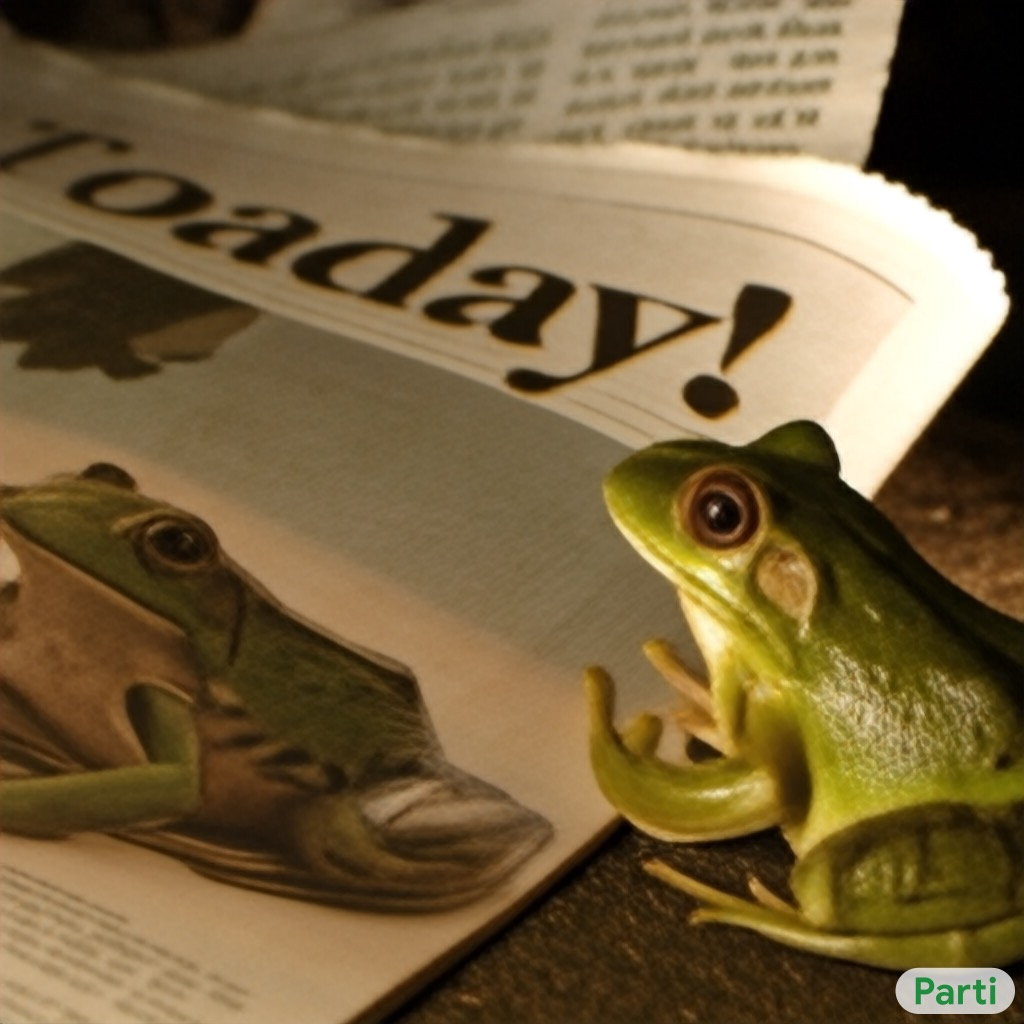
\includegraphics[width=\thirdcolwidth\textwidth]{figures/cherries/frog.jpg}} &&
\multicolumn{6}{c}{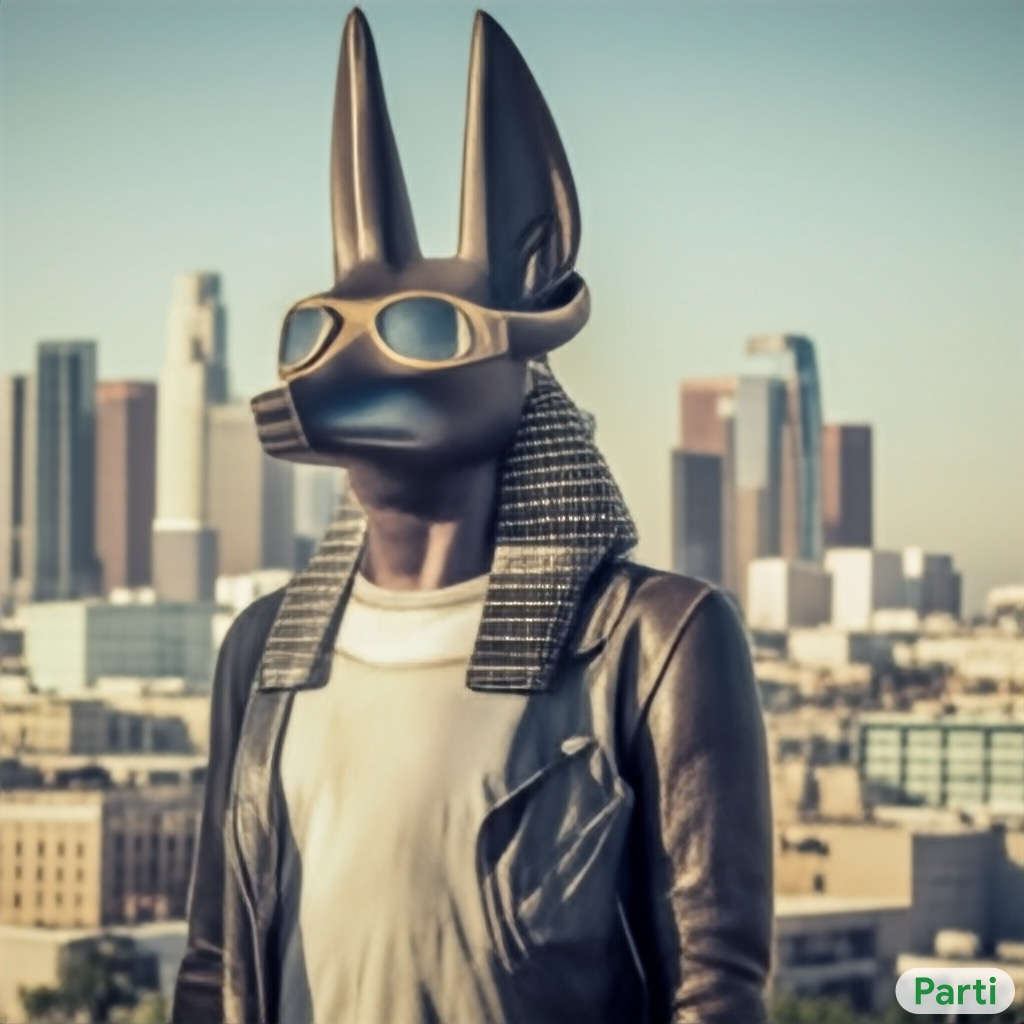
\includegraphics[width=\thirdcolwidth\textwidth]{figures/cherries/anubis_la.jpg}} &&
\multicolumn{6}{c}{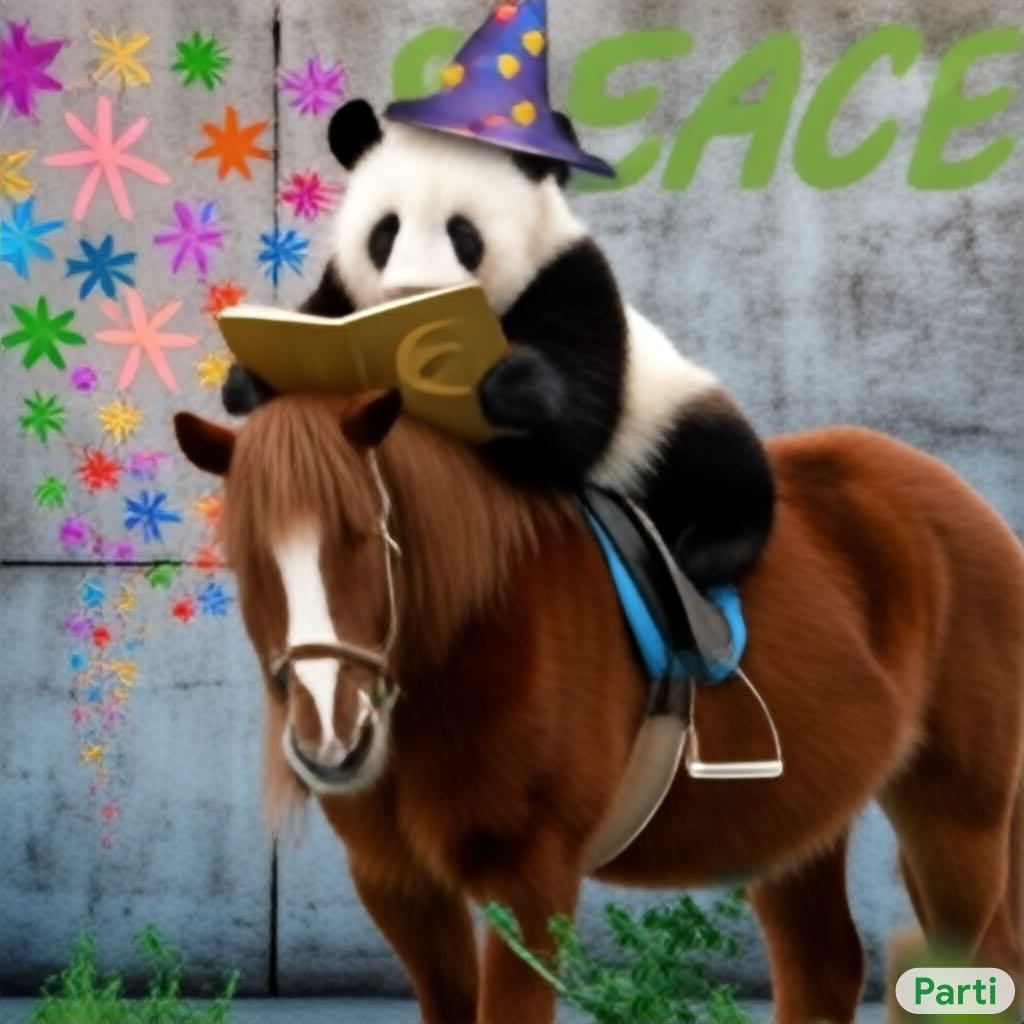
\includegraphics[width=\thirdcolwidth\textwidth]{figures/cherries/panda.jpg}} \\
\multicolumn{6}{p{\thirdcolwidth\textwidth}}{{\tiny \textbf{A}. \textit{A photo of a frog reading the newspaper named ``Toaday'' written on it. There is a frog printed on the newspaper too.}}} && 
\multicolumn{6}{p{\thirdcolwidth\textwidth}}{{\tiny \textbf{B}. \textit{A portrait of a statue of the Egyptian god Anubis wearing aviator goggles, white t-shirt and leather jacket. The city of Los Angeles is in the background. Hi-res DSLR photograph.}}} && 
\multicolumn{6}{p{\thirdcolwidth\textwidth}}{{\tiny \textbf{C}. \textit{A high-contrast photo of a panda riding a horse. The panda is wearing a wizard hat and is reading a book. The horse is standing on a street against a gray concrete wall. Colorful flowers and the word "PEACE" are painted on the wall. Green grass grows from cracks in the street. DSLR photograph. daytime lighting.}}} \\

\multicolumn{3}{c}{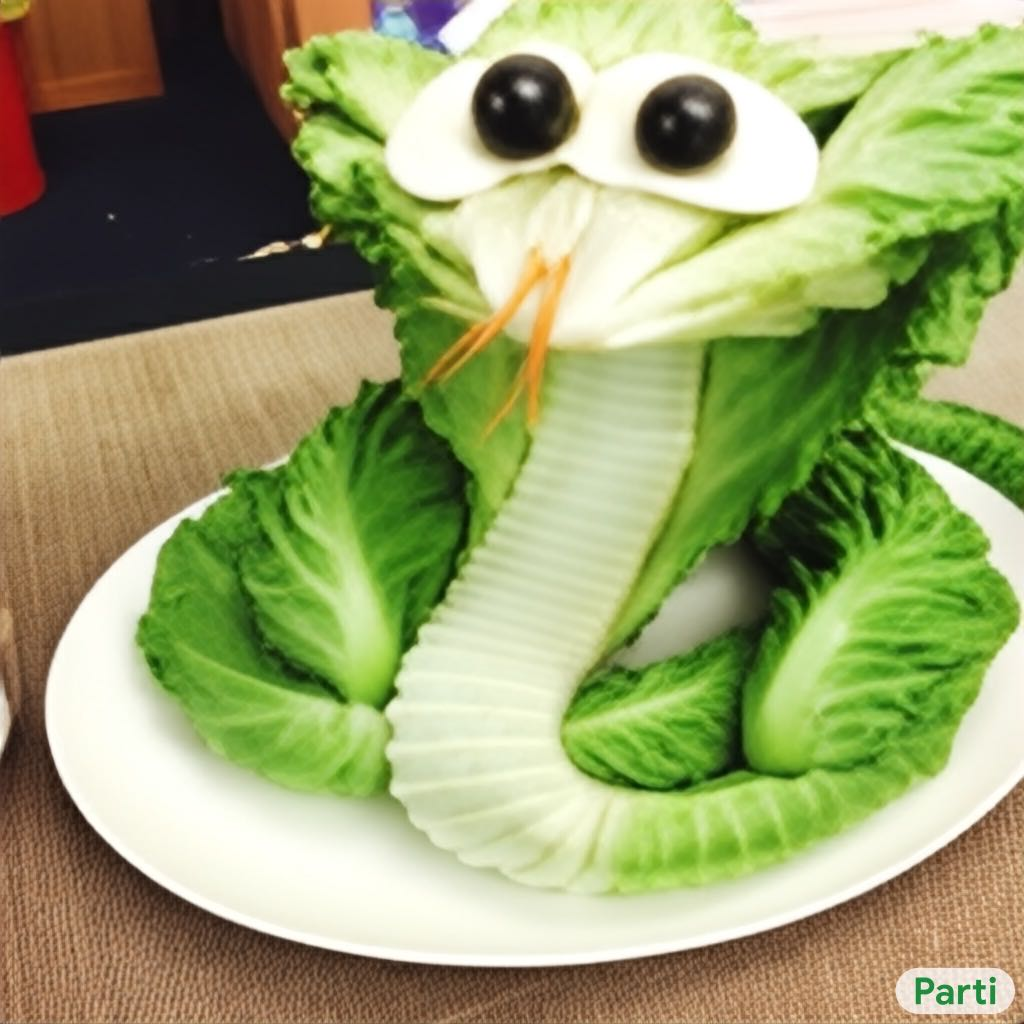
\includegraphics[width=\twobytwocolwidth\textwidth]{figures/cherries/snake_salad.jpg}} &
\multicolumn{3}{c}{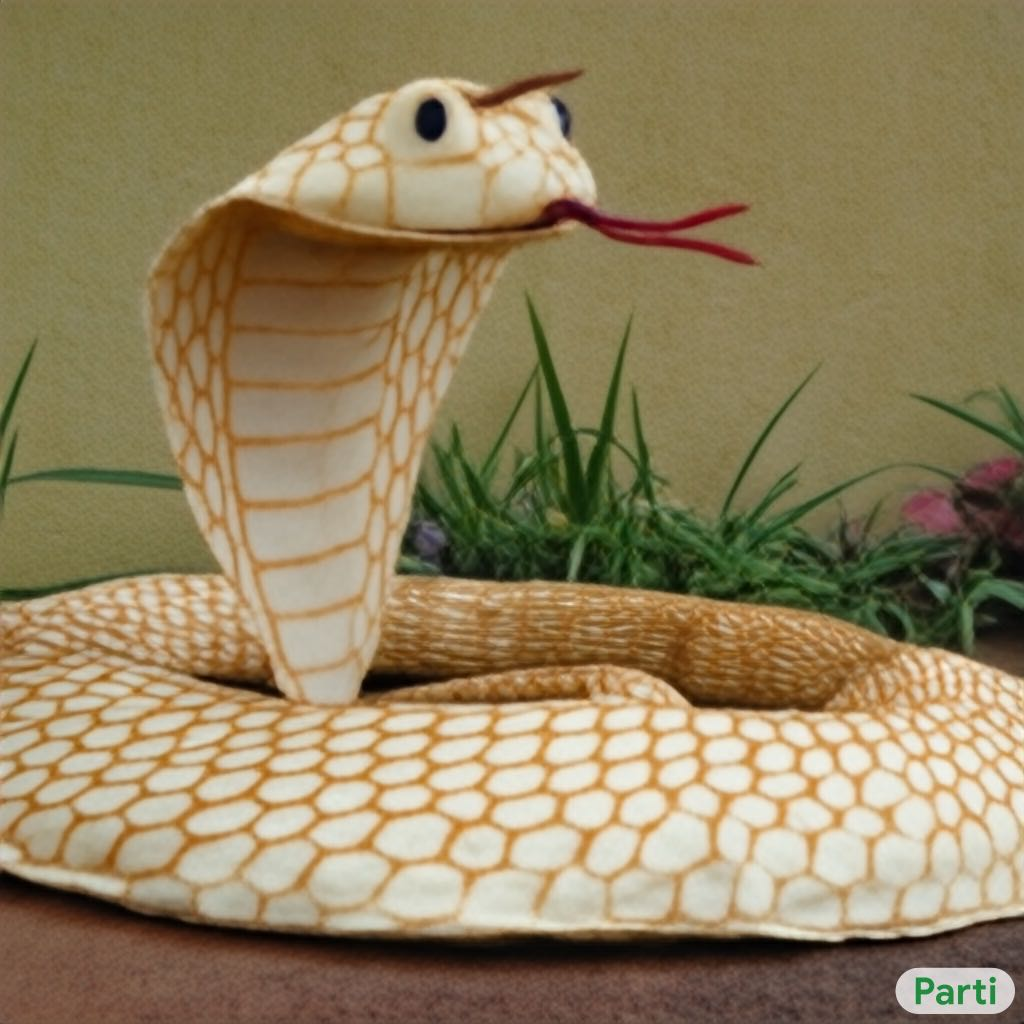
\includegraphics[width=\twobytwocolwidth\textwidth]{figures/cherries/snake_pancake.jpg}} &&
\multicolumn{3}{c}{
\includegraphics[width=\twobytwocolwidth\textwidth]{figures/cherries/wombat1.jpg}} &
\multicolumn{3}{c}{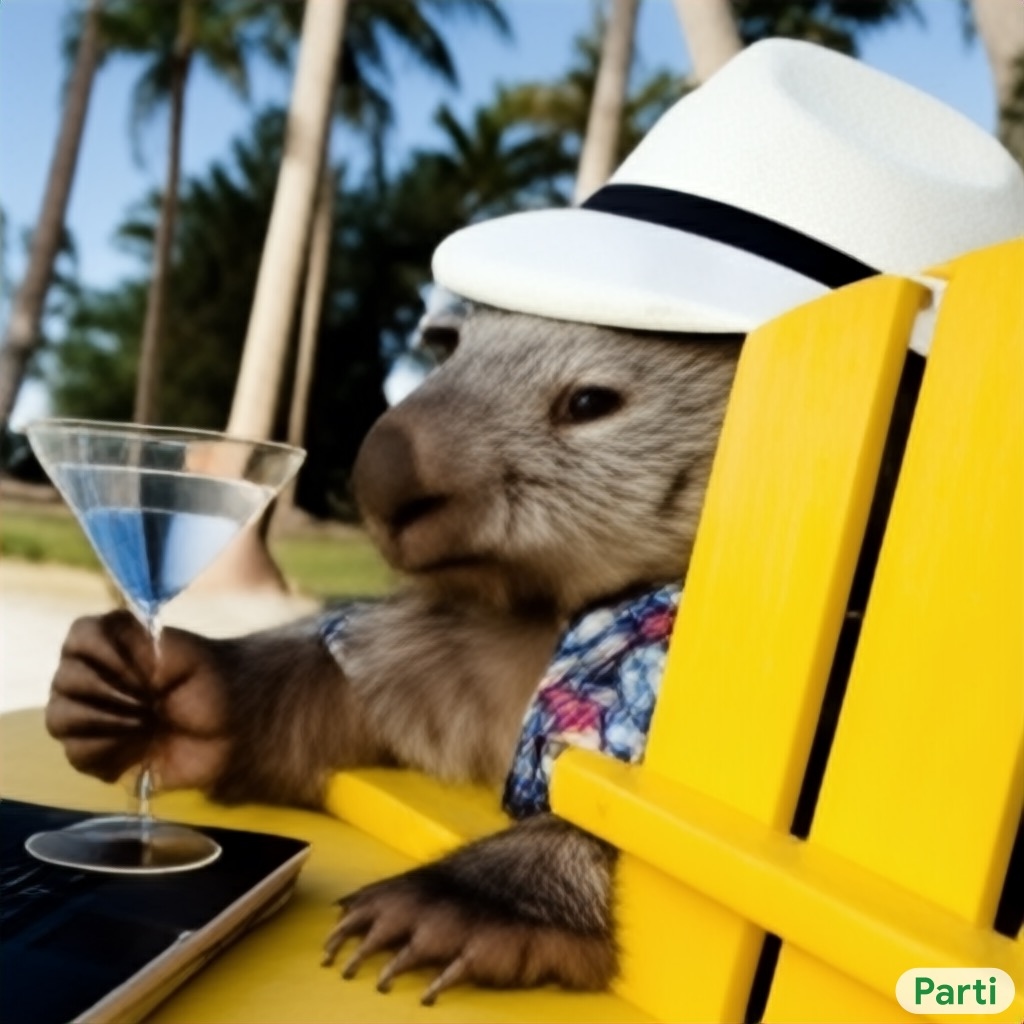
\includegraphics[width=\twobytwocolwidth\textwidth]{figures/cherries/wombat2.jpg}} &&
\multicolumn{3}{c}{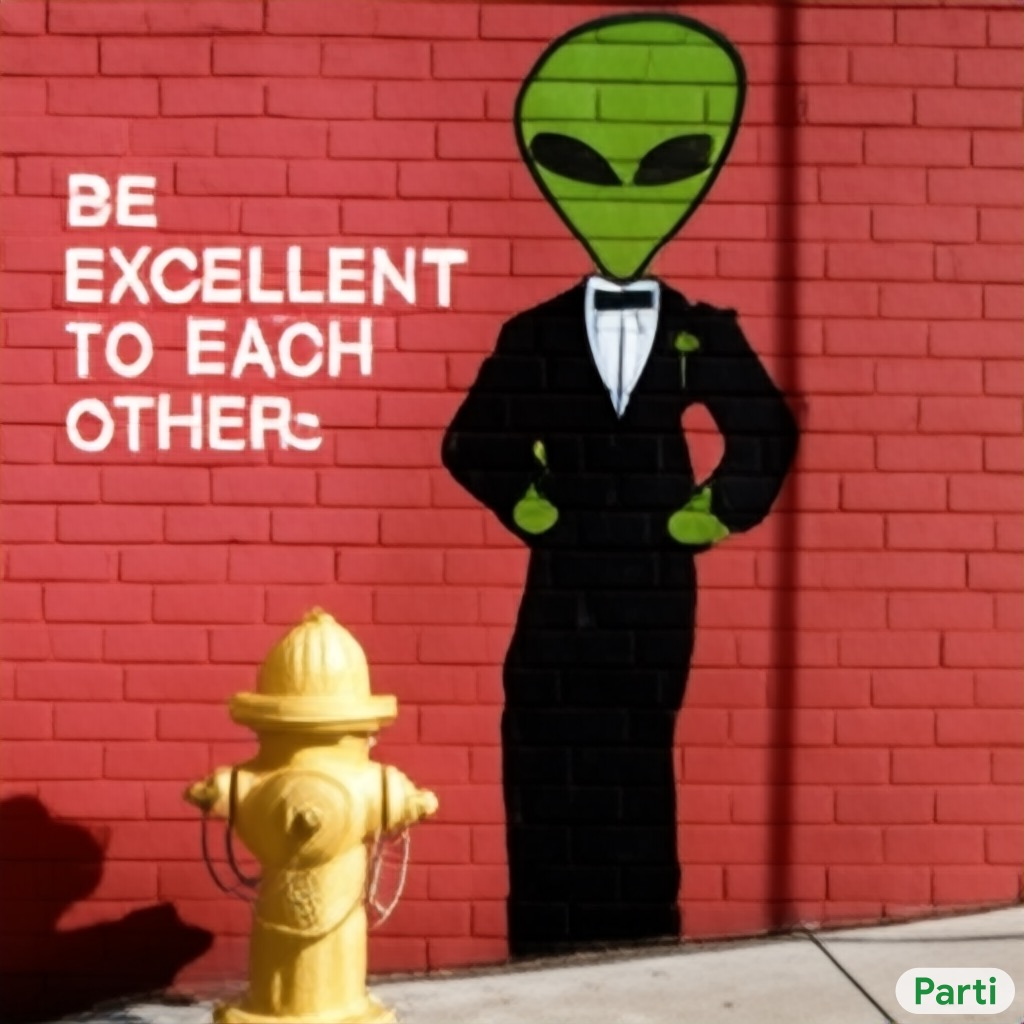
\includegraphics[width=\twobytwocolwidth\textwidth]{figures/cherries/excellent_alien.jpg}} &
\multicolumn{3}{c}{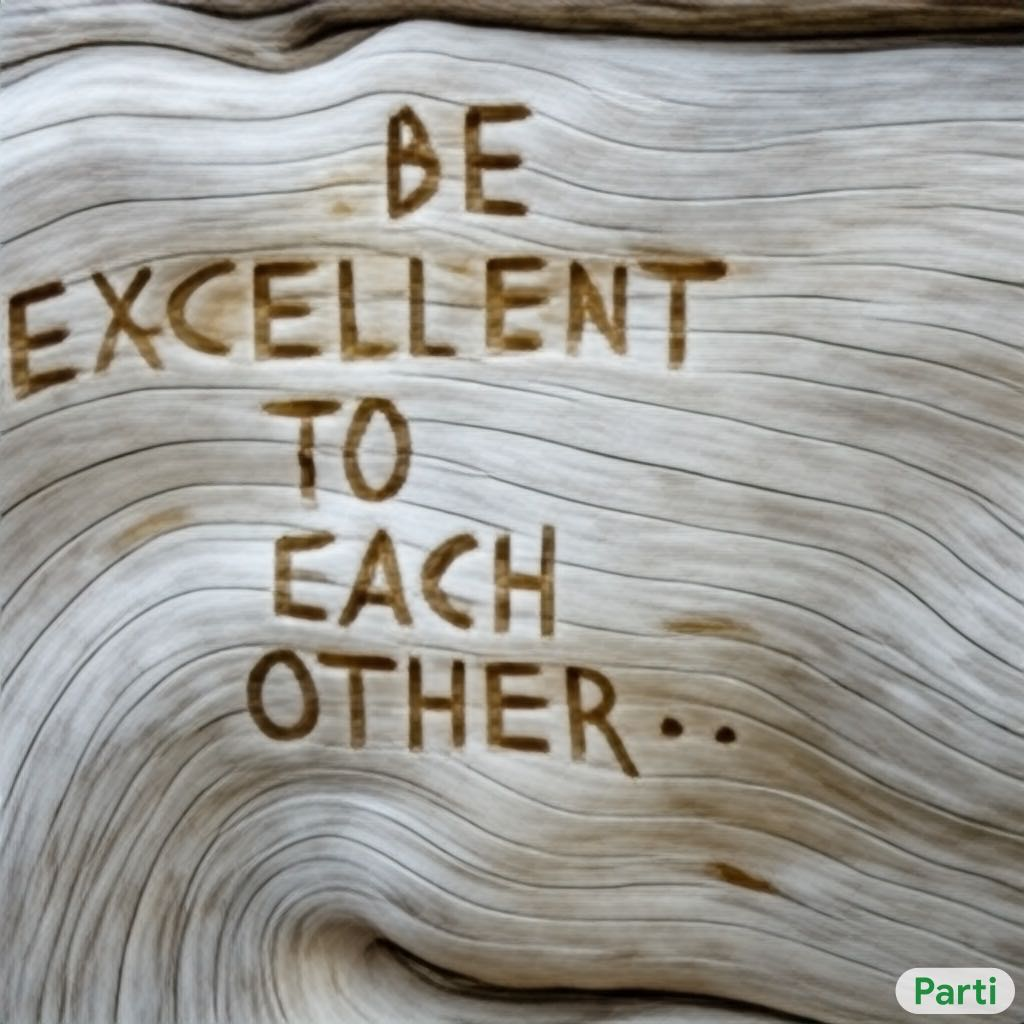
\includegraphics[width=\twobytwocolwidth\textwidth]{figures/cherries/excellent_wood.jpg}} \\

\multicolumn{3}{c}{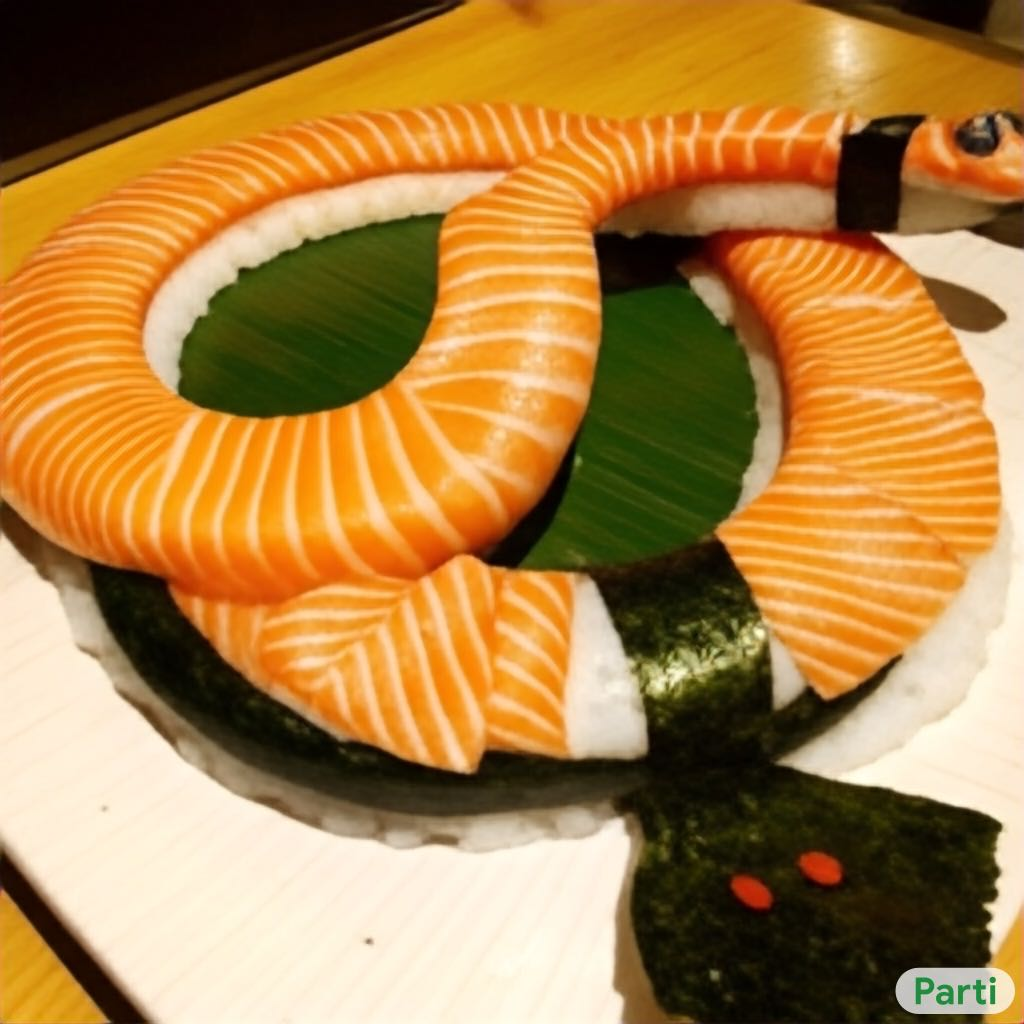
\includegraphics[width=\twobytwocolwidth\textwidth]{figures/cherries/snake_sushi.jpg}} &
\multicolumn{3}{c}{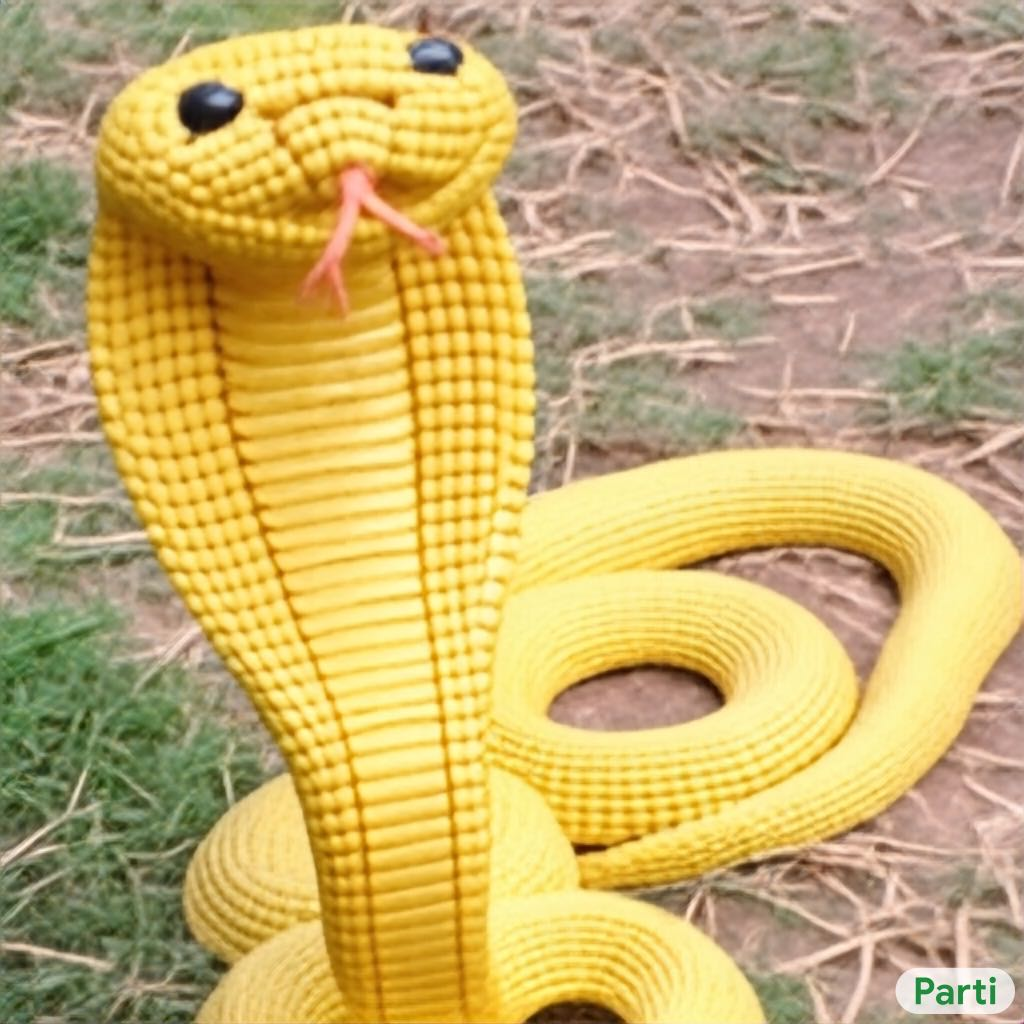
\includegraphics[width=\twobytwocolwidth\textwidth]{figures/cherries/snake_corn.jpg}} &&
\multicolumn{3}{c}{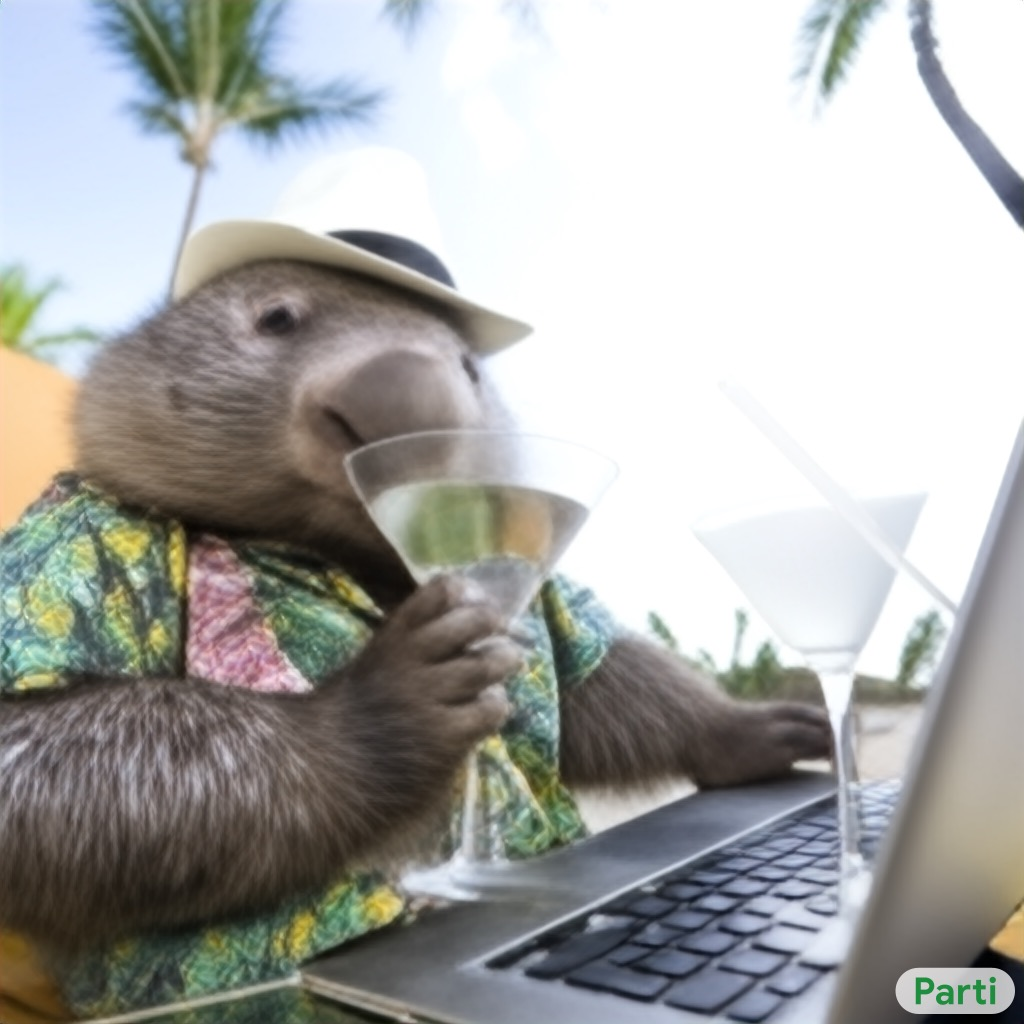
\includegraphics[width=\twobytwocolwidth\textwidth]{figures/cherries/wombat3.jpg}} &
\multicolumn{3}{c}{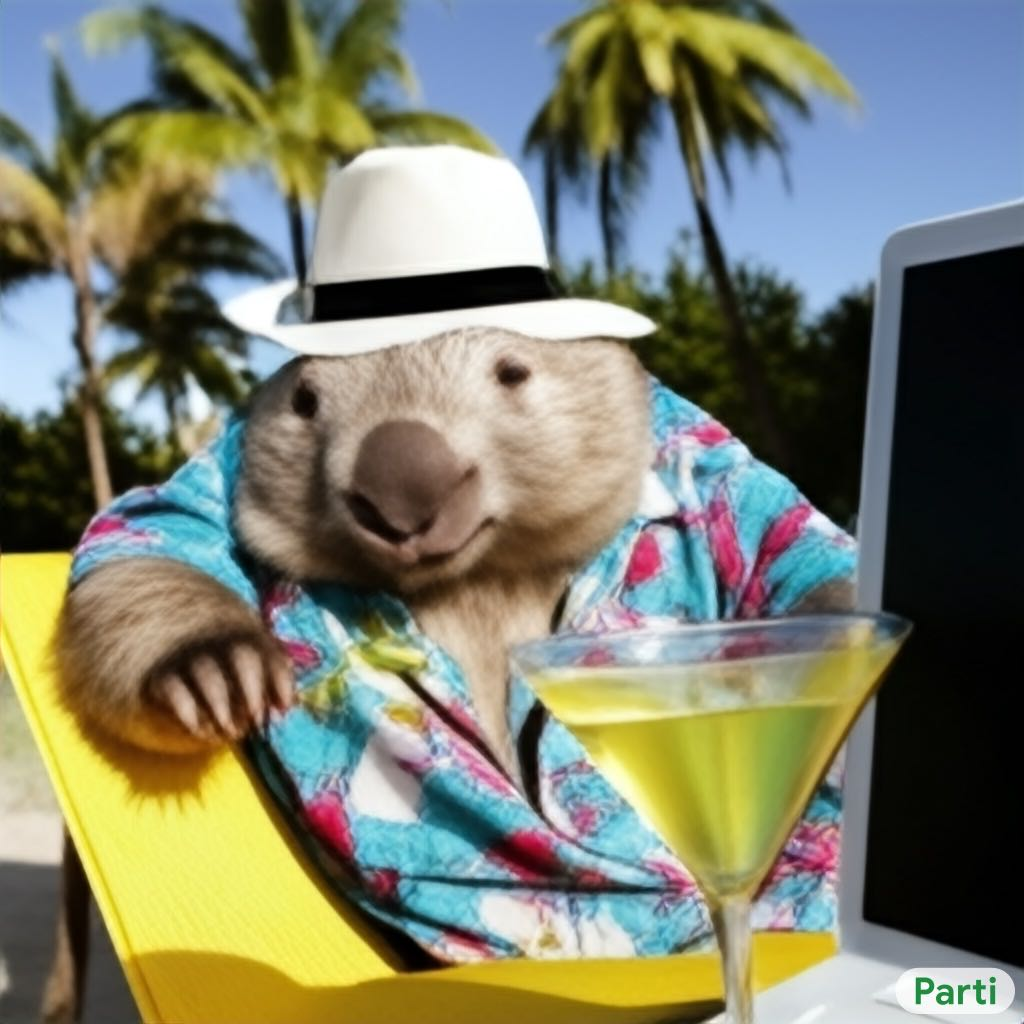
\includegraphics[width=\twobytwocolwidth\textwidth]{figures/cherries/wombat4.jpg}} &&
\multicolumn{3}{c}{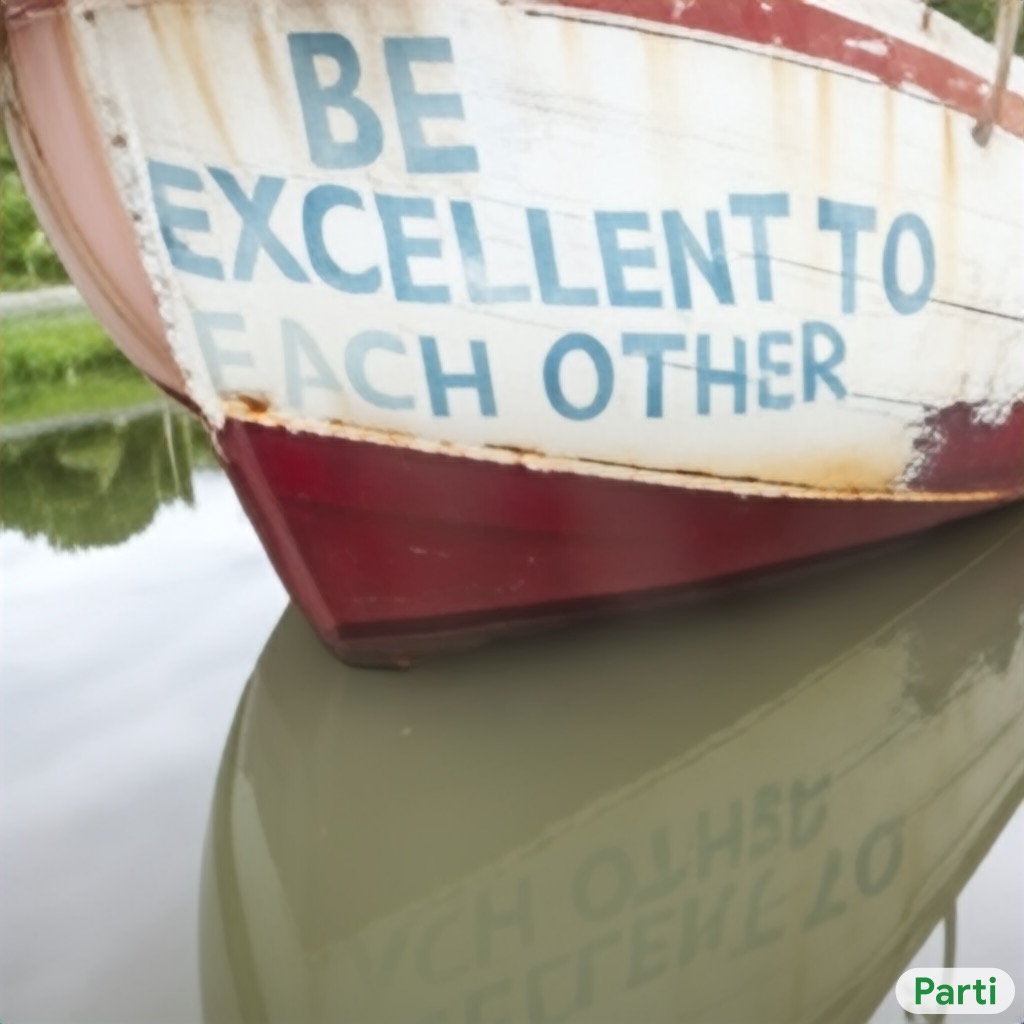
\includegraphics[width=\twobytwocolwidth\textwidth]{figures/cherries/excellent_boat.jpg}} &
\multicolumn{3}{c}{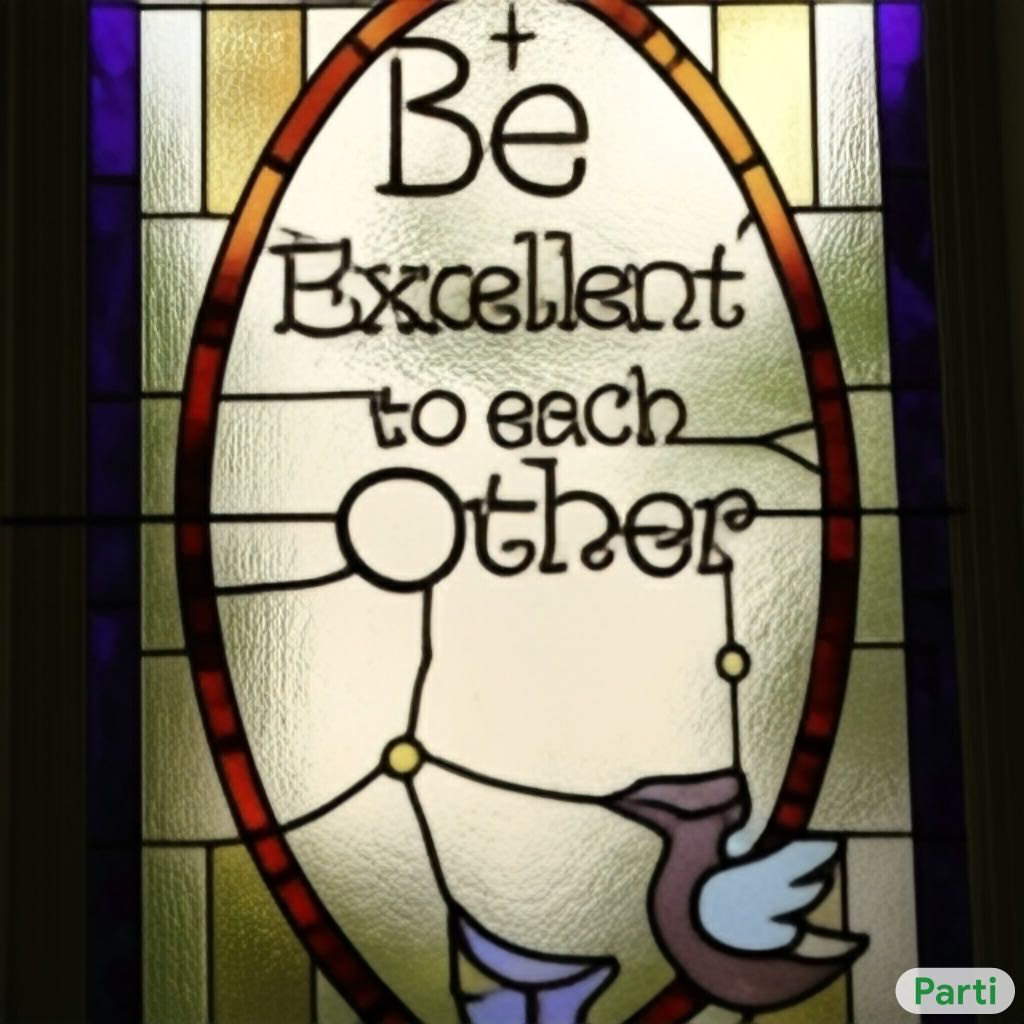
\includegraphics[width=\twobytwocolwidth\textwidth]{figures/cherries/excellent_glass.jpg}} \\
\multicolumn{6}{p{\thirdcolwidth\textwidth}}{{\tiny \textbf{D}. \textit{A giant cobra snake made from X.} \textit{X} $\in$ \{\textit{``salad'', ``pancakes'', ``sushi'', ``corn''}\}}} &&
\multicolumn{6}{p{\thirdcolwidth\textwidth}}{{\tiny \textbf{E}. \textit{A wombat sits in a yellow beach chair, while sipping a martini that is on his laptop keyboard. The wombat is wearing a white panama hat and a floral Hawaiian shirt. Out-of-focus palm trees in the background. DSLR photograph. Wide-angle view.}}} &&
\multicolumn{6}{p{\thirdcolwidth\textwidth}}{{\tiny \textbf{F}. \textit{The saying "BE EXCELLENT TO EACH OTHER" ...}, (a) brick wall and alien (b) driftwood. (c) old wooden boat with reflection. (d) stained glass. (See text for full prompts.)}} \\

\multicolumn{2}{c}{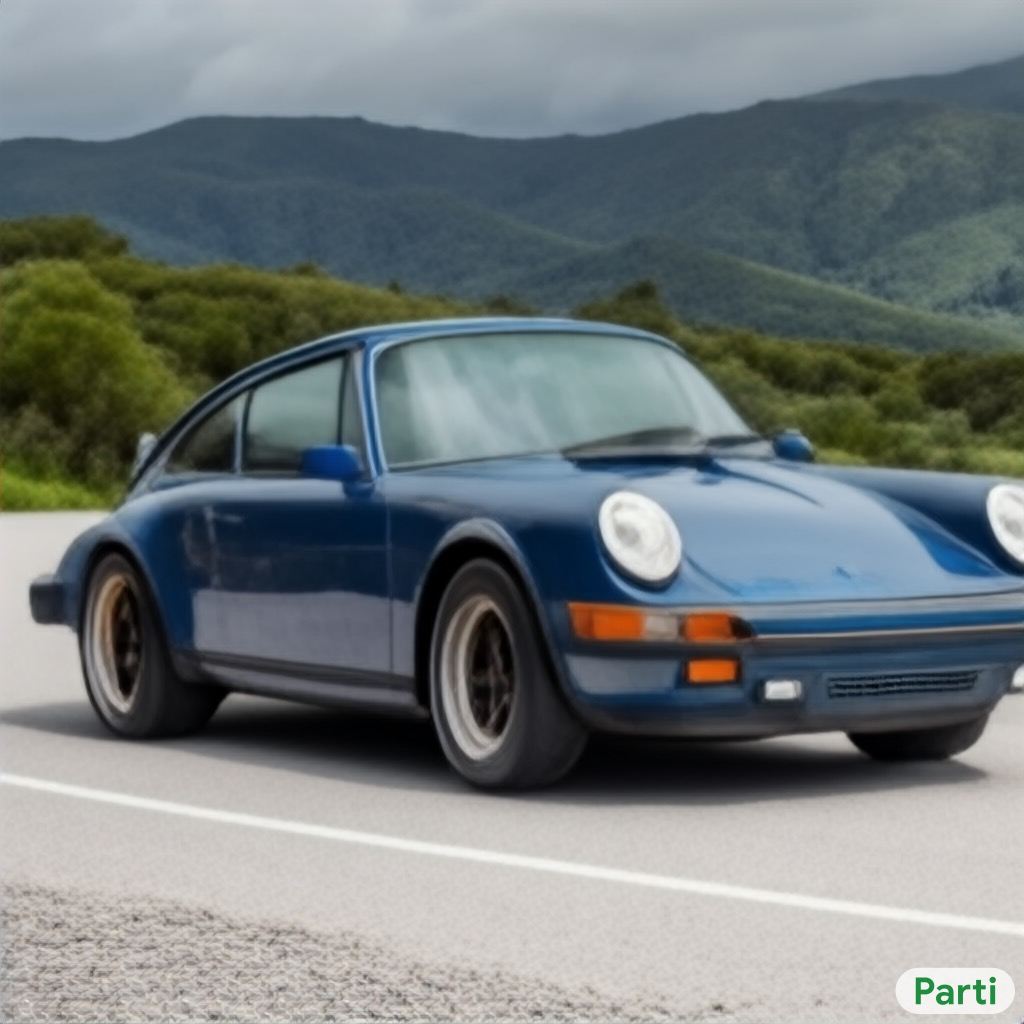
\includegraphics[width=\threebythreecolwidth\textwidth]{figures/cherries/porsche1977.jpg}} &
\multicolumn{2}{c}{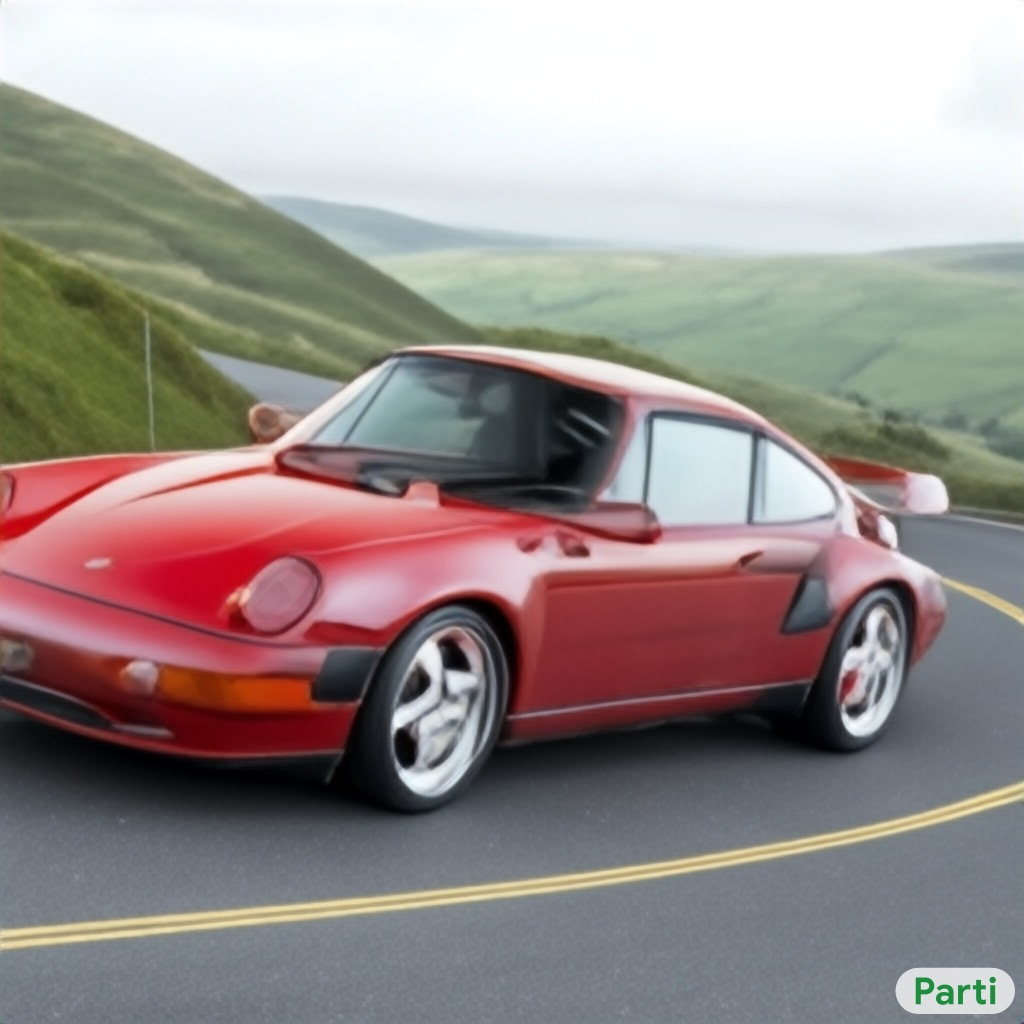
\includegraphics[width=\threebythreecolwidth\textwidth]{figures/cherries/porsche1997.jpg}} &
\multicolumn{2}{c}{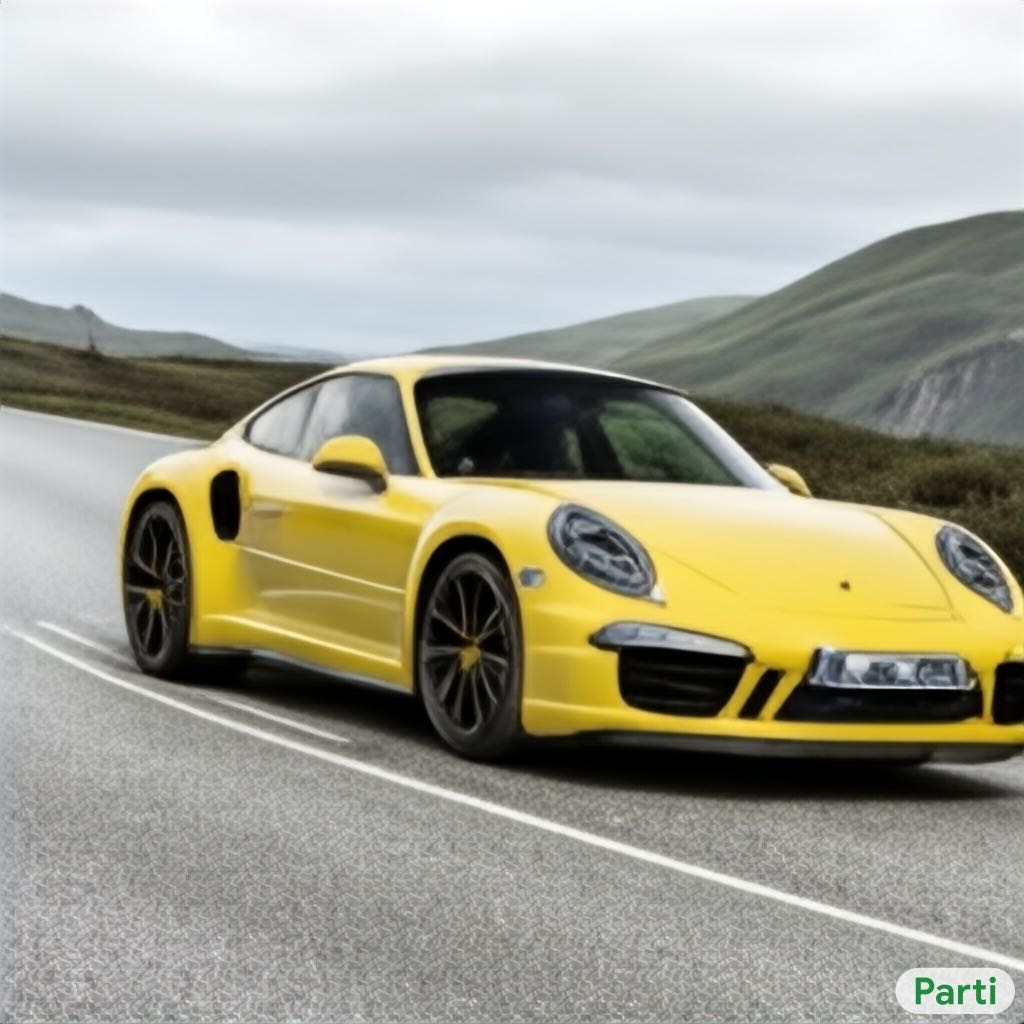
\includegraphics[width=\threebythreecolwidth\textwidth]{figures/cherries/porsche2017.jpg}} &&
\multicolumn{2}{c}{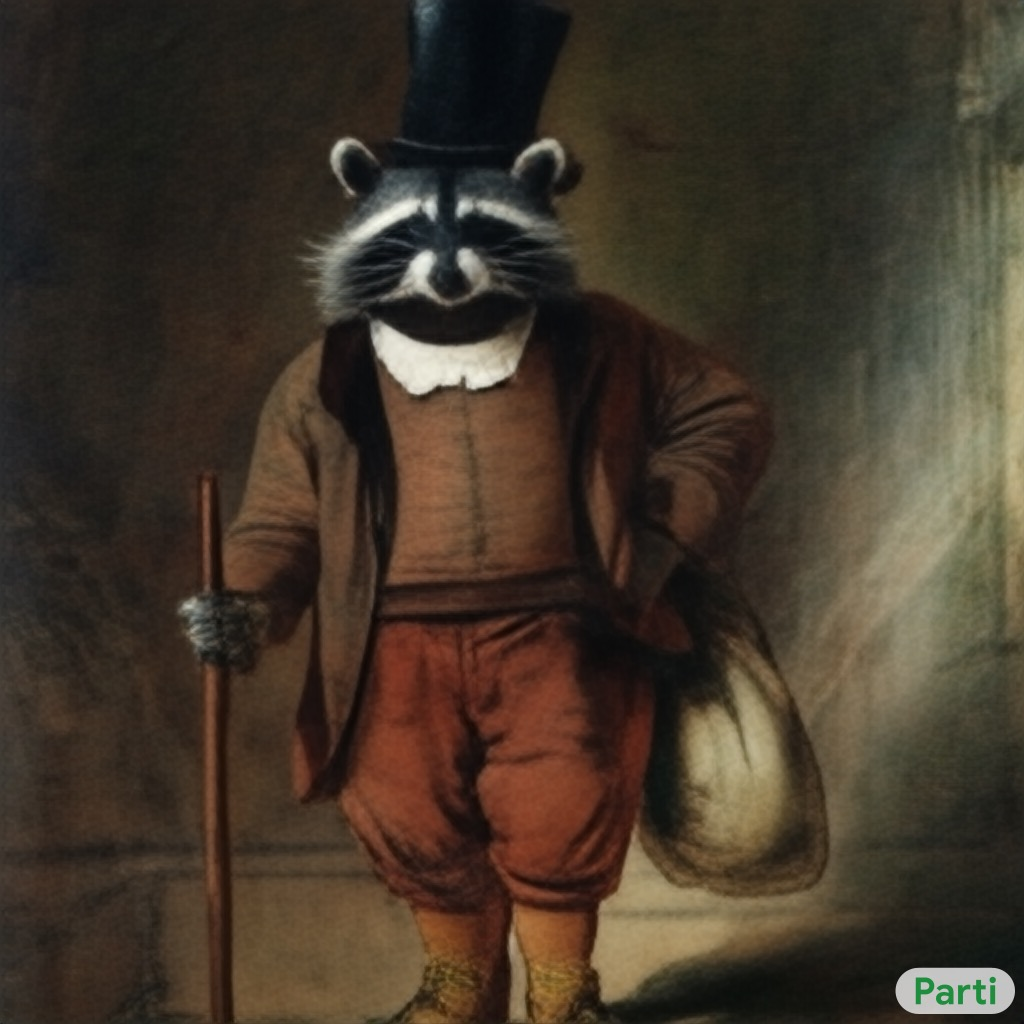
\includegraphics[width=\threebythreecolwidth\textwidth]{figures/cherries/rembrandt.jpg}} &
\multicolumn{2}{c}{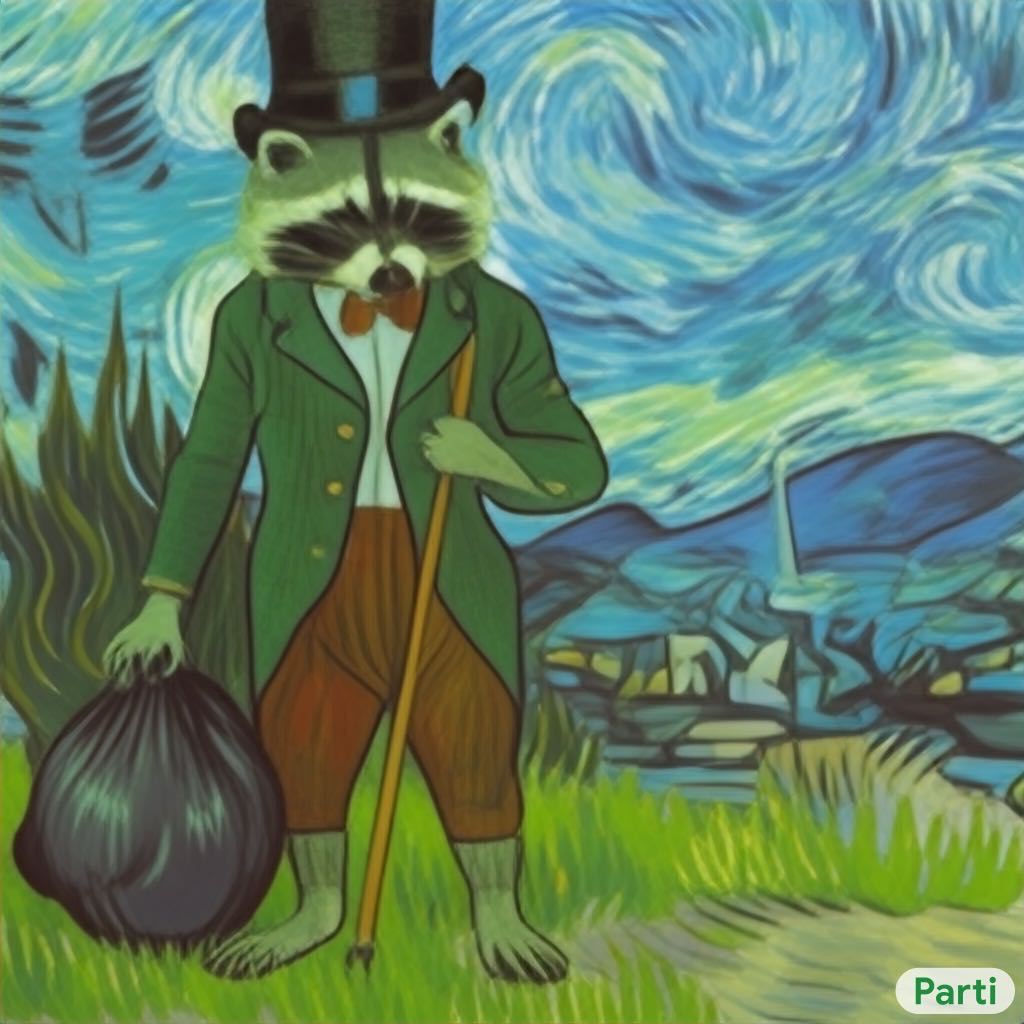
\includegraphics[width=\threebythreecolwidth\textwidth]{figures/cherries/vangogh.jpg}} &
\multicolumn{2}{c}{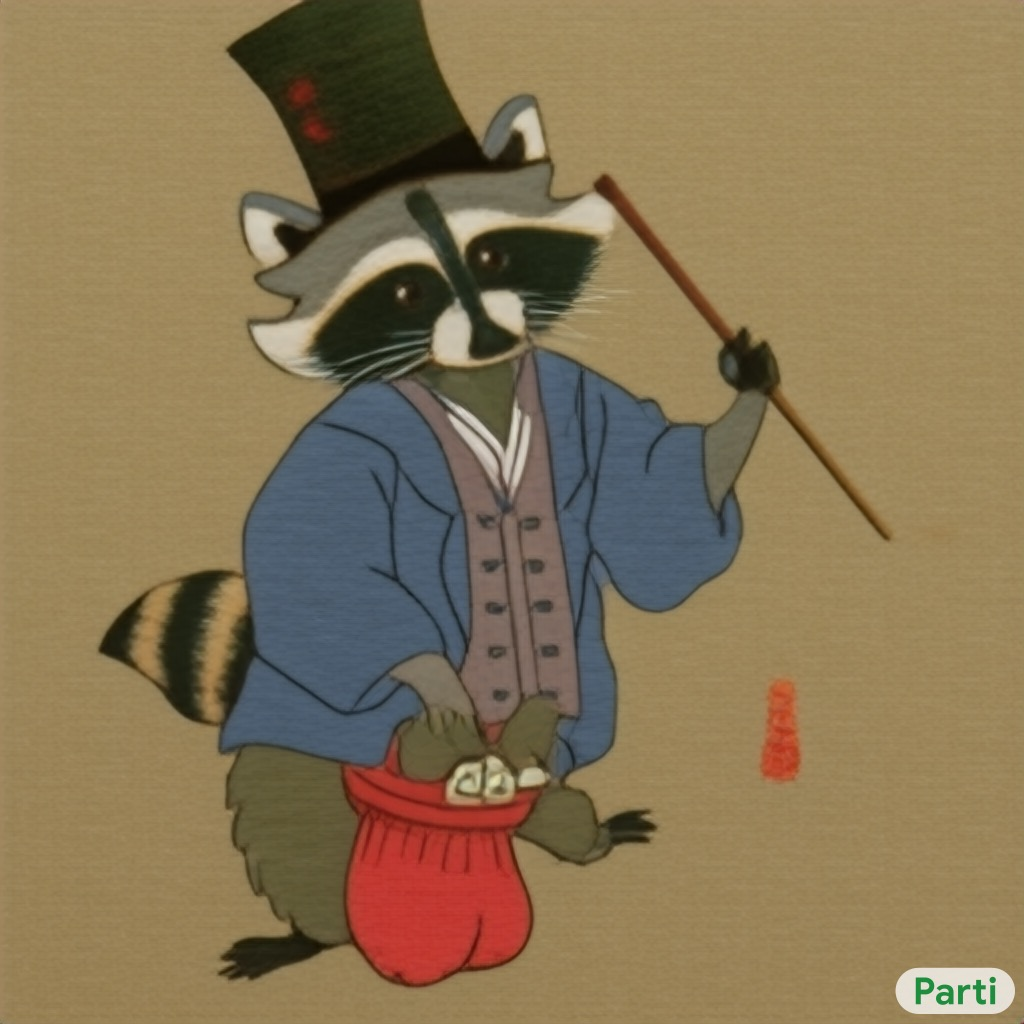
\includegraphics[width=\threebythreecolwidth\textwidth]{figures/cherries/hokusai.jpg}} &&
\multicolumn{2}{c}{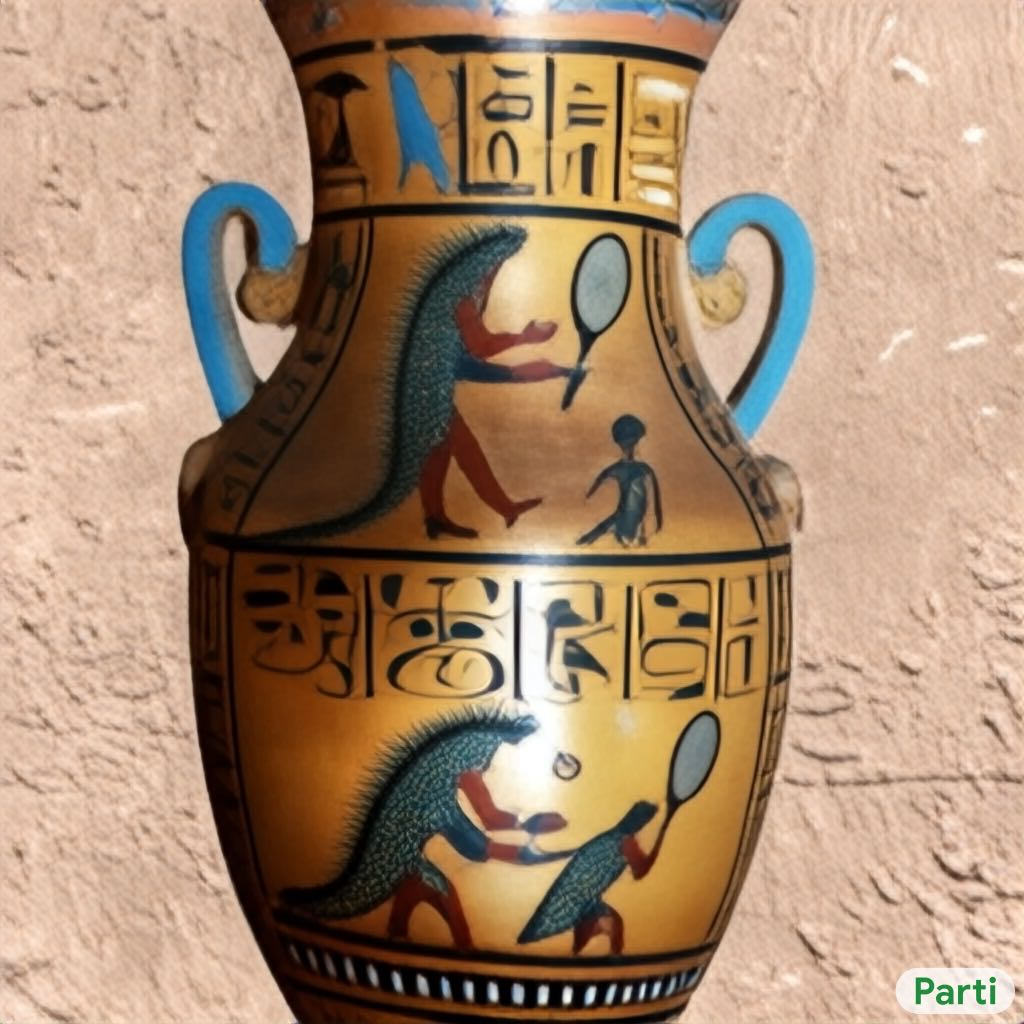
\includegraphics[width=\threebythreecolwidth\textwidth]{figures/cherries/pangolin_tennis.jpg}} &
\multicolumn{2}{c}{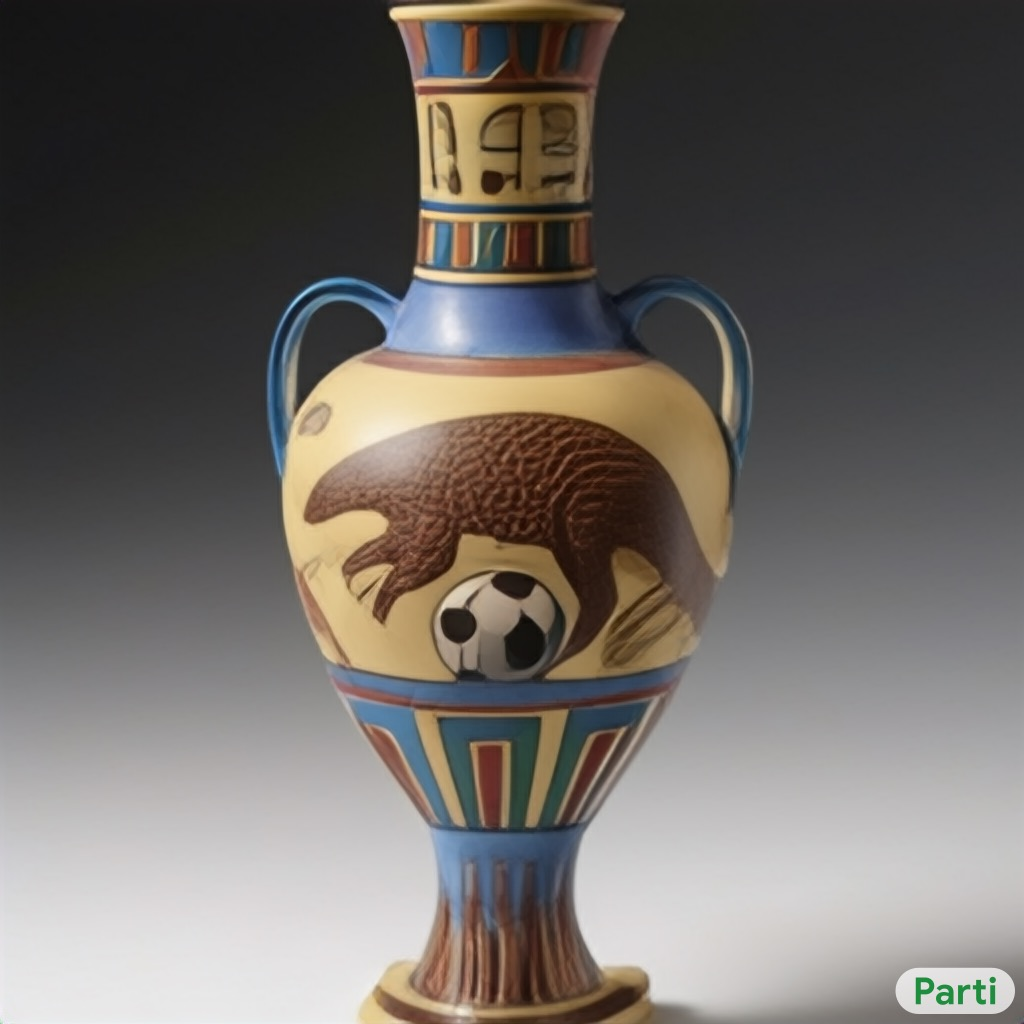
\includegraphics[width=\threebythreecolwidth\textwidth]{figures/cherries/pangolin_soccer.jpg}} &
\multicolumn{2}{c}{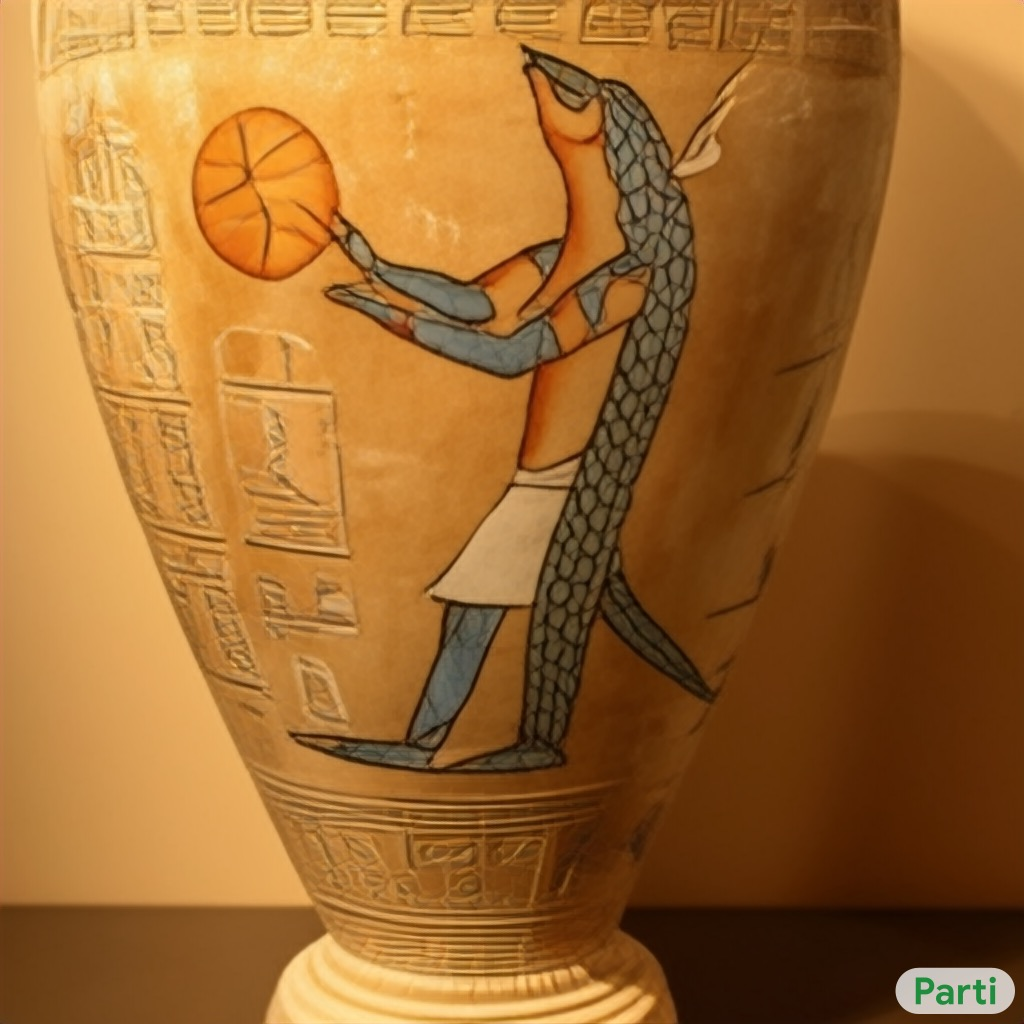
\includegraphics[width=\threebythreecolwidth\textwidth]{figures/cherries/pangolin_basketball.jpg}}\\

\multicolumn{2}{c}{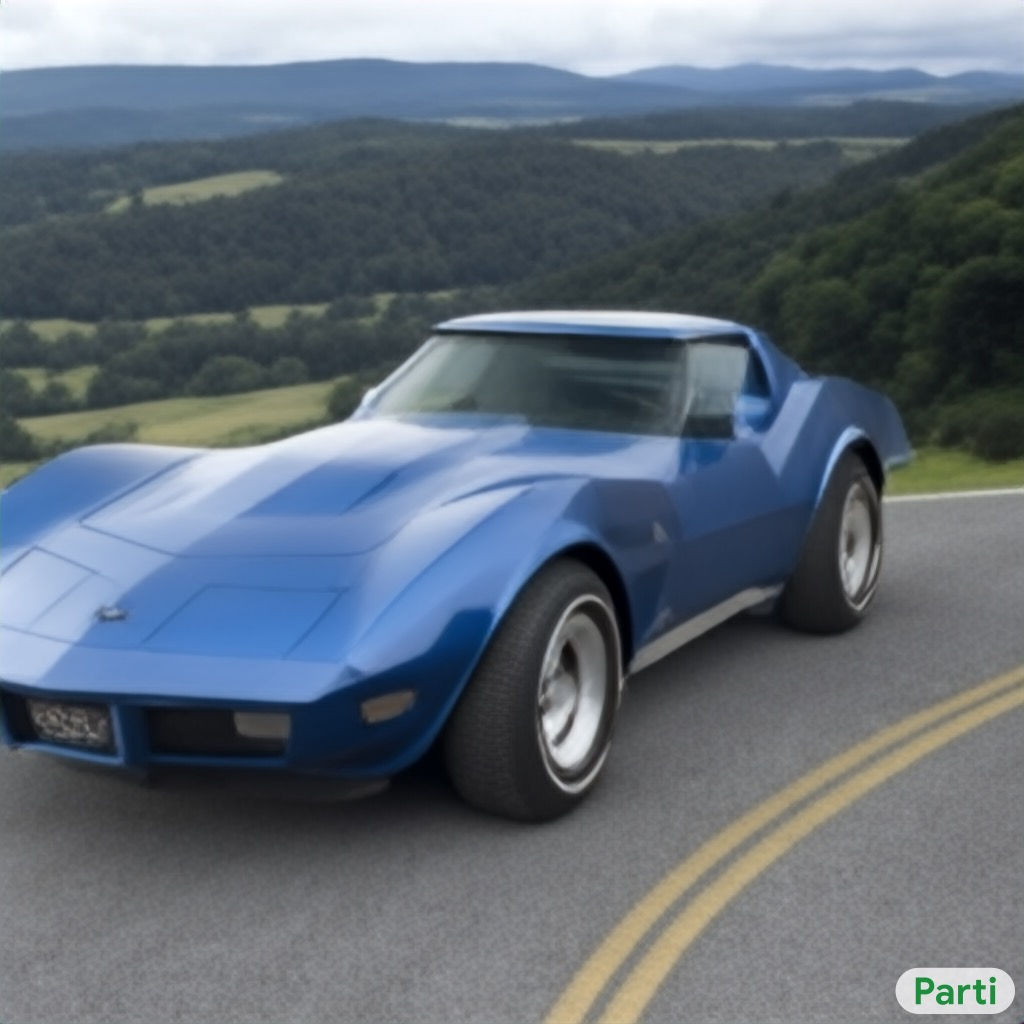
\includegraphics[width=\threebythreecolwidth\textwidth]{figures/cherries/corvette1977.jpg}} &
\multicolumn{2}{c}{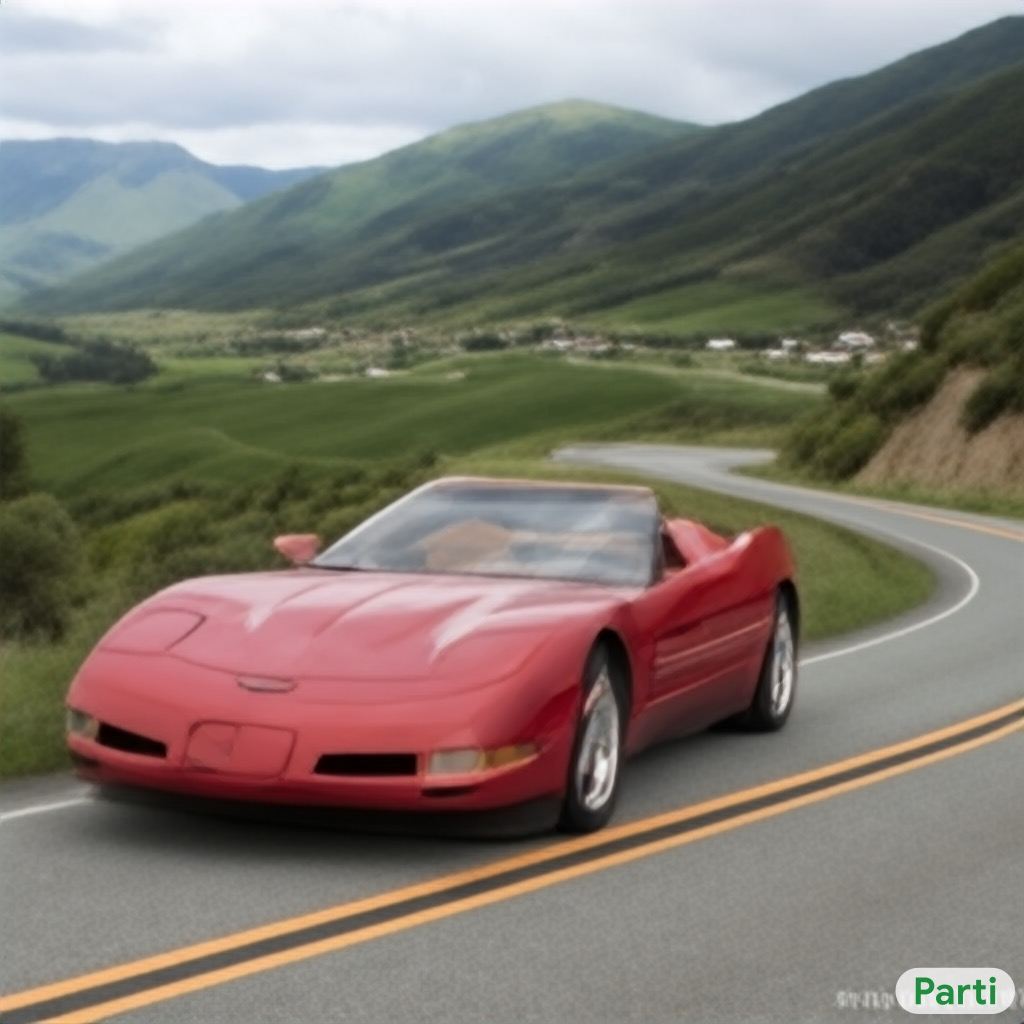
\includegraphics[width=\threebythreecolwidth\textwidth]{figures/cherries/corvette1997.jpg}} &
\multicolumn{2}{c}{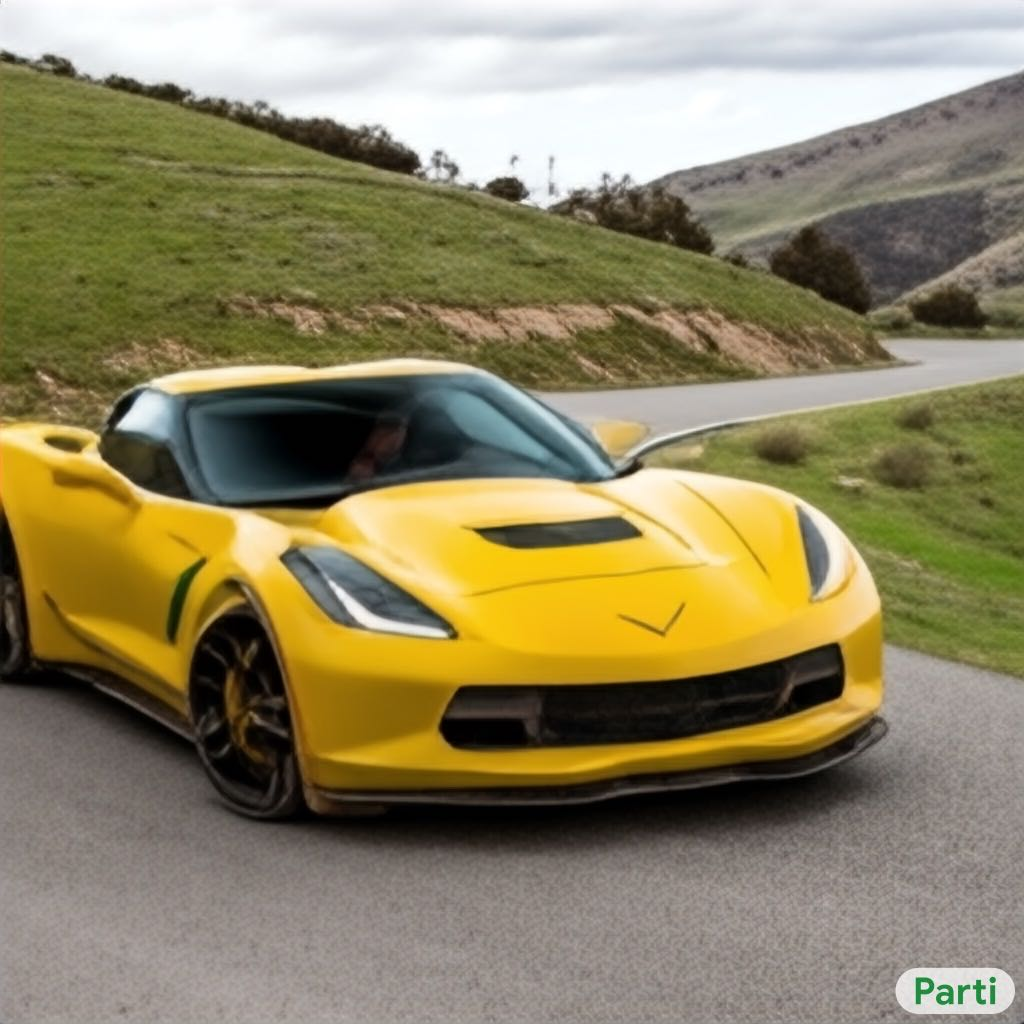
\includegraphics[width=\threebythreecolwidth\textwidth]{figures/cherries/corvette2017.jpg}} &&
\multicolumn{2}{c}{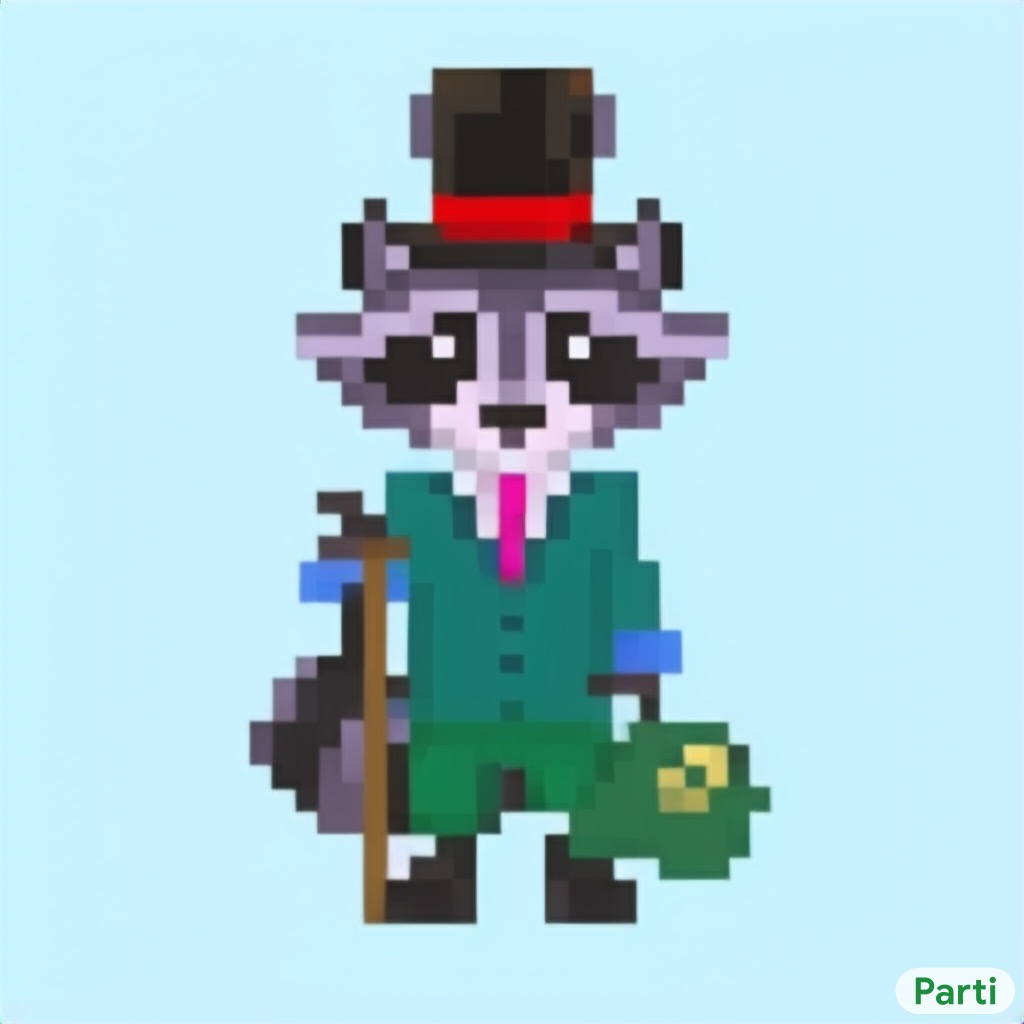
\includegraphics[width=\threebythreecolwidth\textwidth]{figures/cherries/pixelart.jpg}} &
\multicolumn{2}{c}{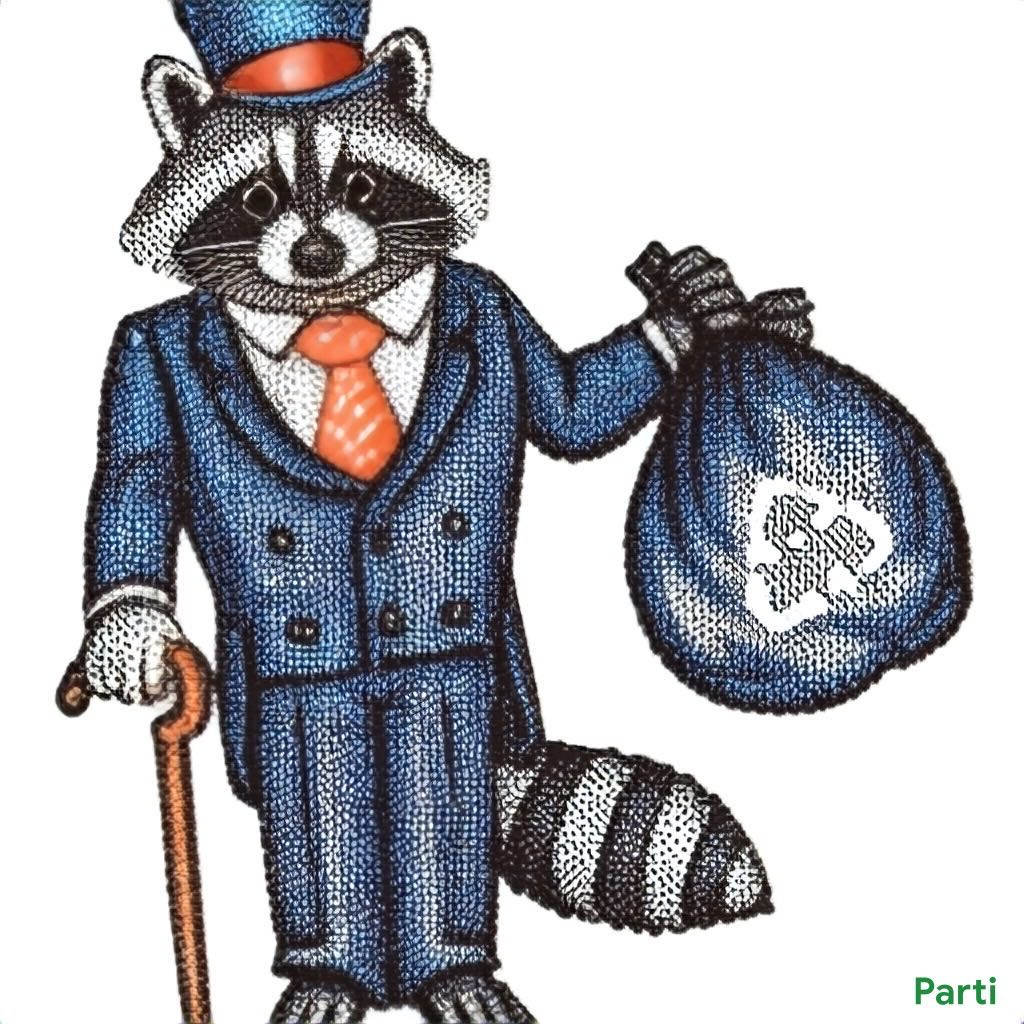
\includegraphics[width=\threebythreecolwidth\textwidth]{figures/cherries/pointilism.jpg}} &
\multicolumn{2}{c}{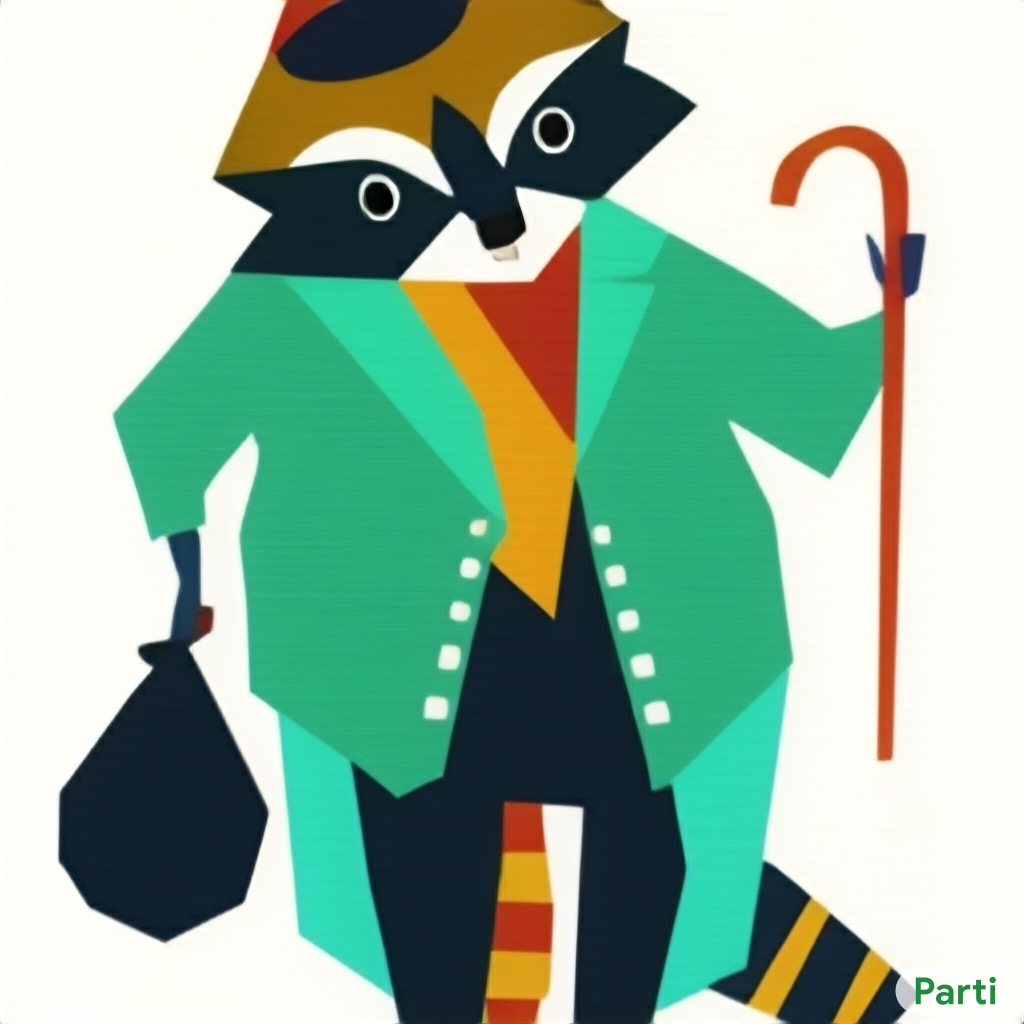
\includegraphics[width=\threebythreecolwidth\textwidth]{figures/cherries/cubism.jpg}} &&
\multicolumn{2}{c}{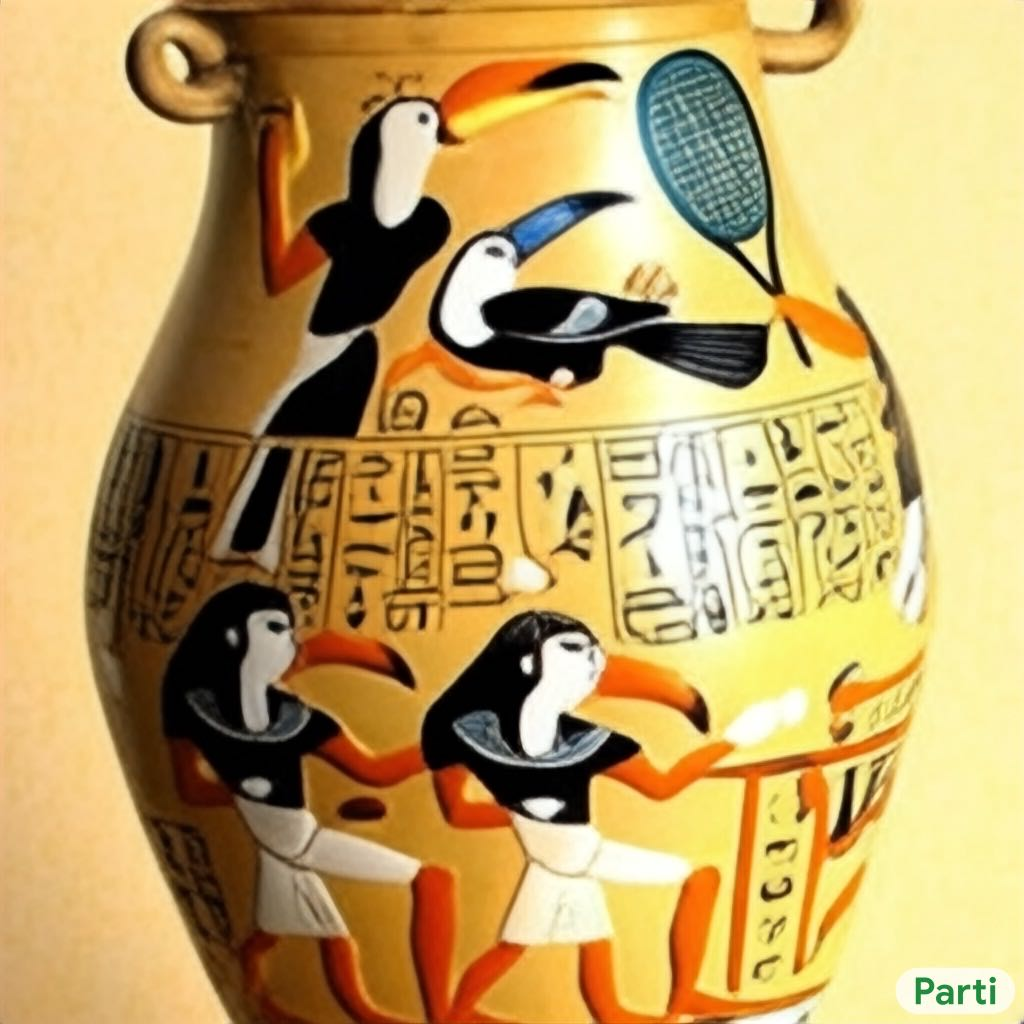
\includegraphics[width=\threebythreecolwidth\textwidth]{figures/cherries/toucan_tennis.jpg}} &
\multicolumn{2}{c}{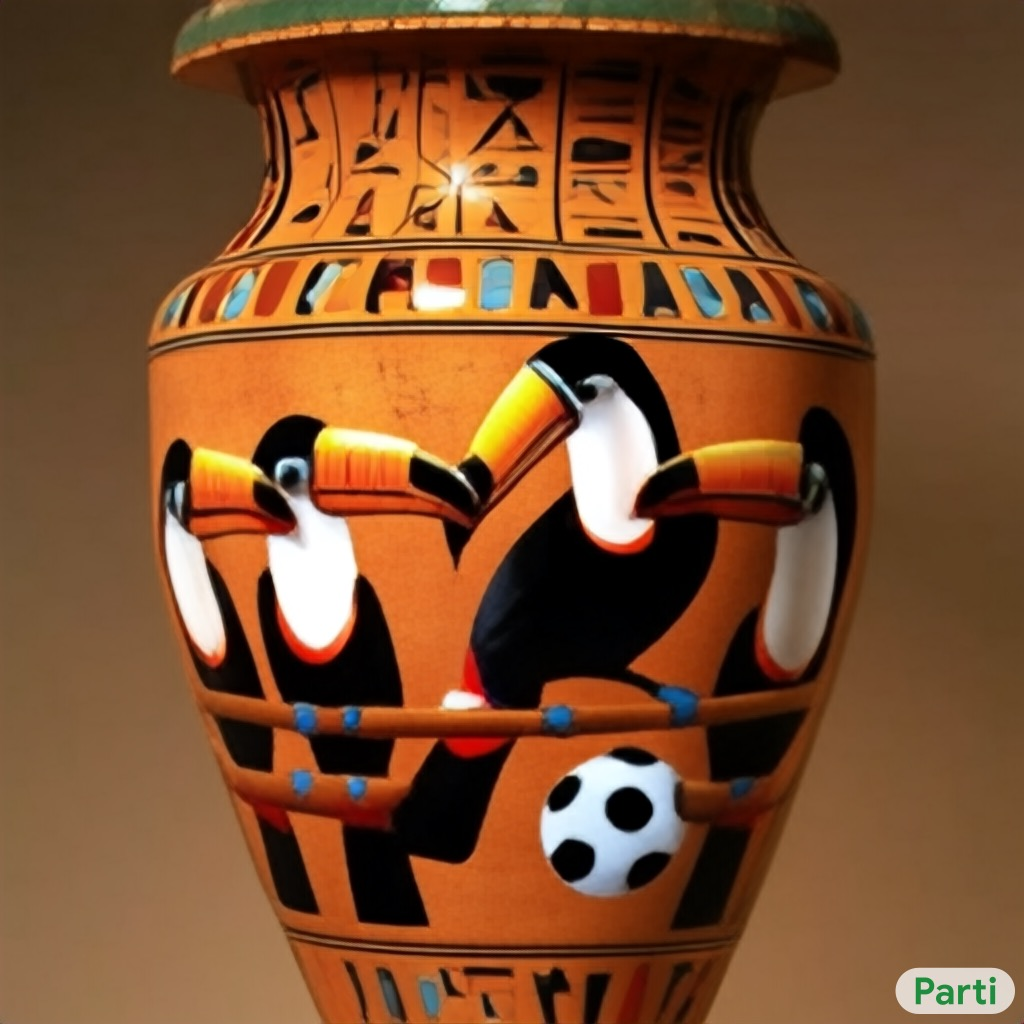
\includegraphics[width=\threebythreecolwidth\textwidth]{figures/cherries/toucan_soccer.jpg}} &
\multicolumn{2}{c}{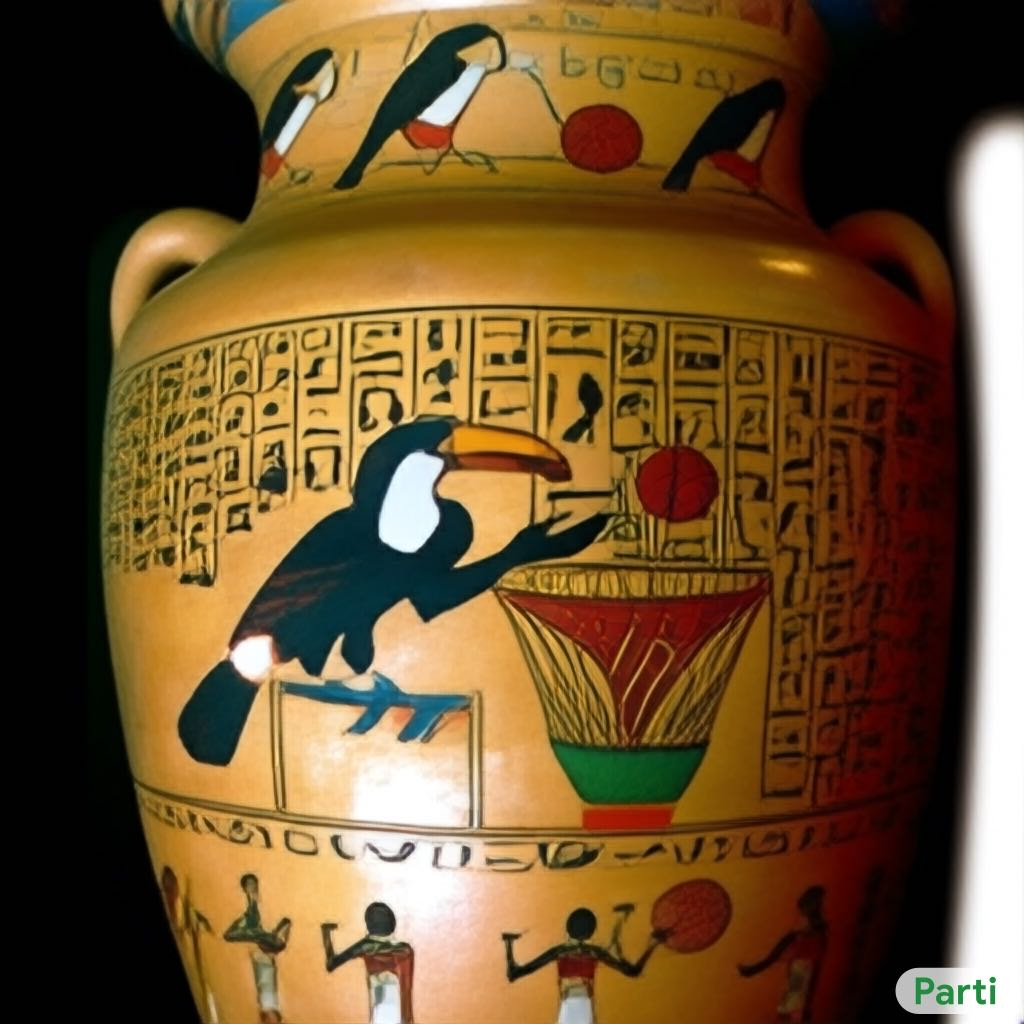
\includegraphics[width=\threebythreecolwidth\textwidth]{figures/cherries/toucan_basketball.jpg}}\\

\multicolumn{2}{c}{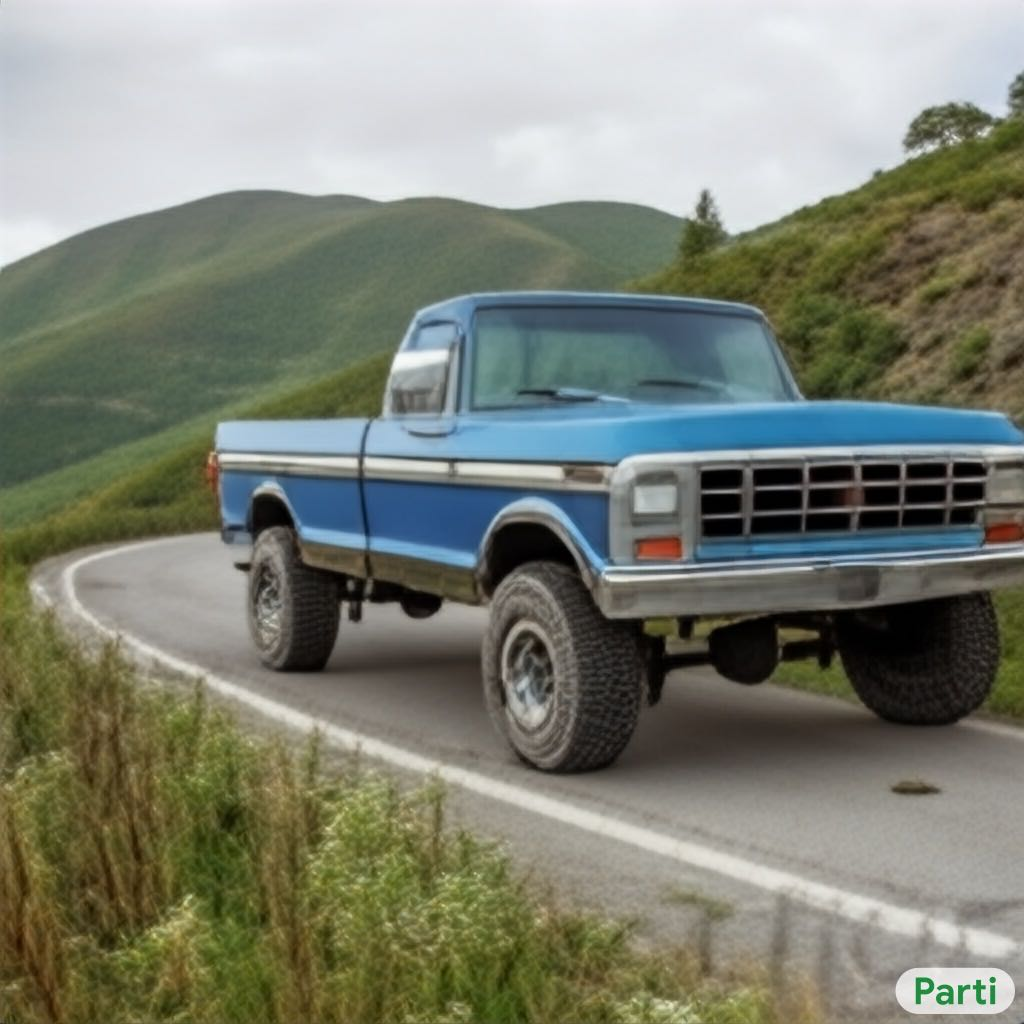
\includegraphics[width=\threebythreecolwidth\textwidth]{figures/cherries/ford1977.jpg}} &
\multicolumn{2}{c}{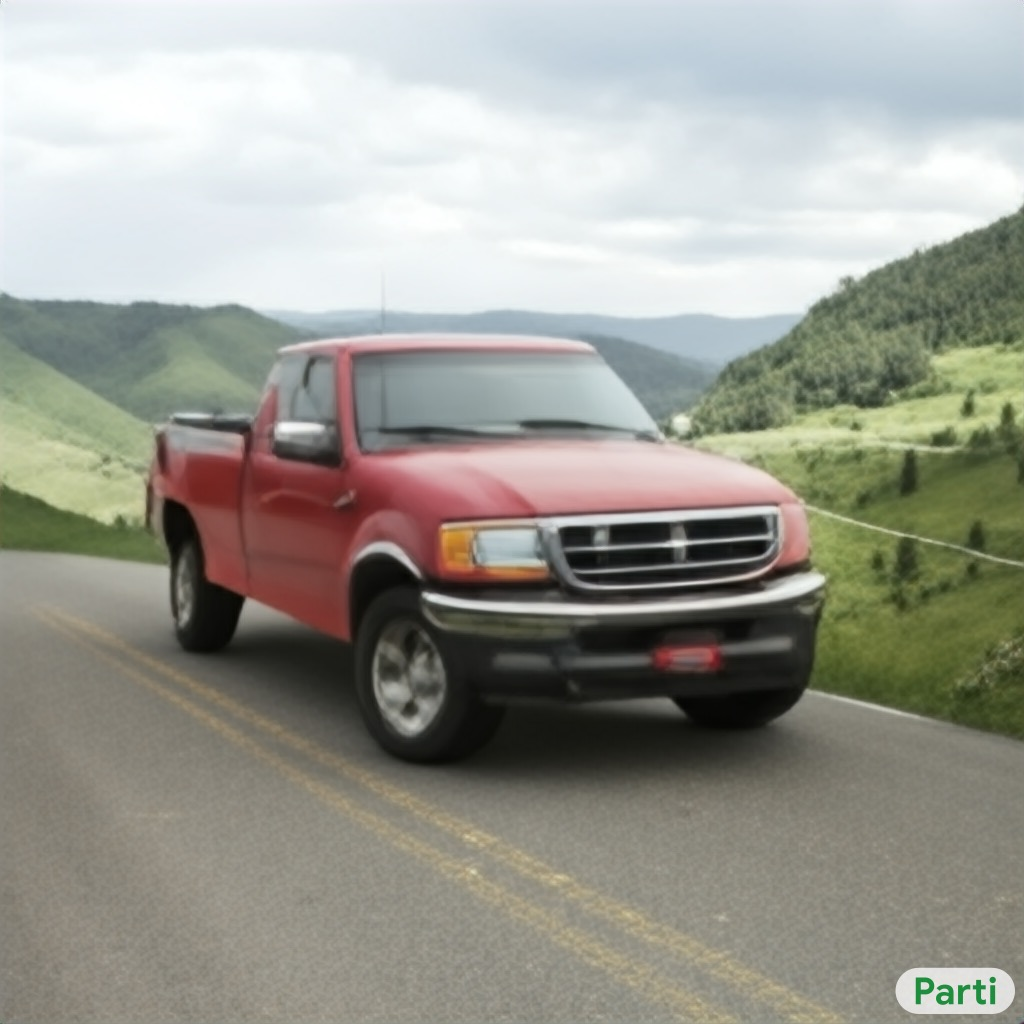
\includegraphics[width=\threebythreecolwidth\textwidth]{figures/cherries/ford1997.jpg}} &
\multicolumn{2}{c}{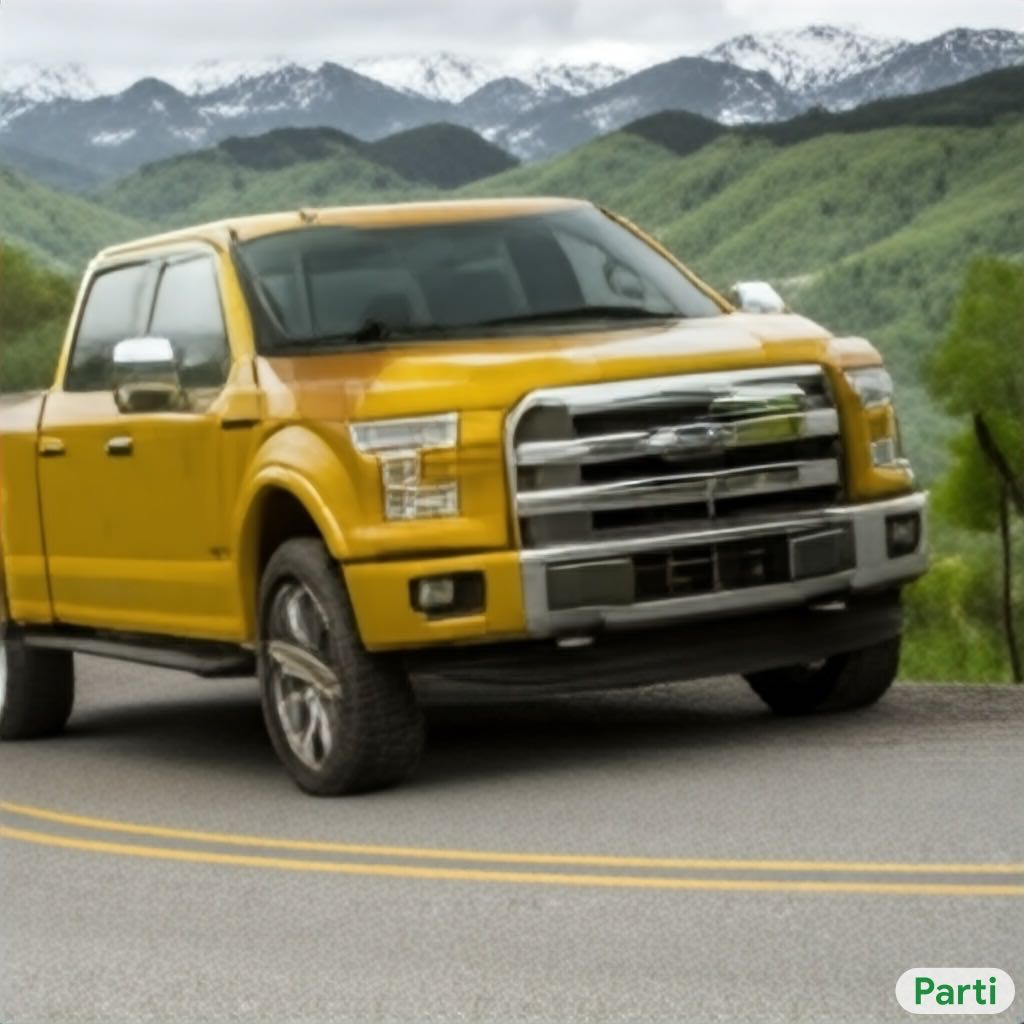
\includegraphics[width=\threebythreecolwidth\textwidth]{figures/cherries/ford2017.jpg}} &&
\multicolumn{2}{c}{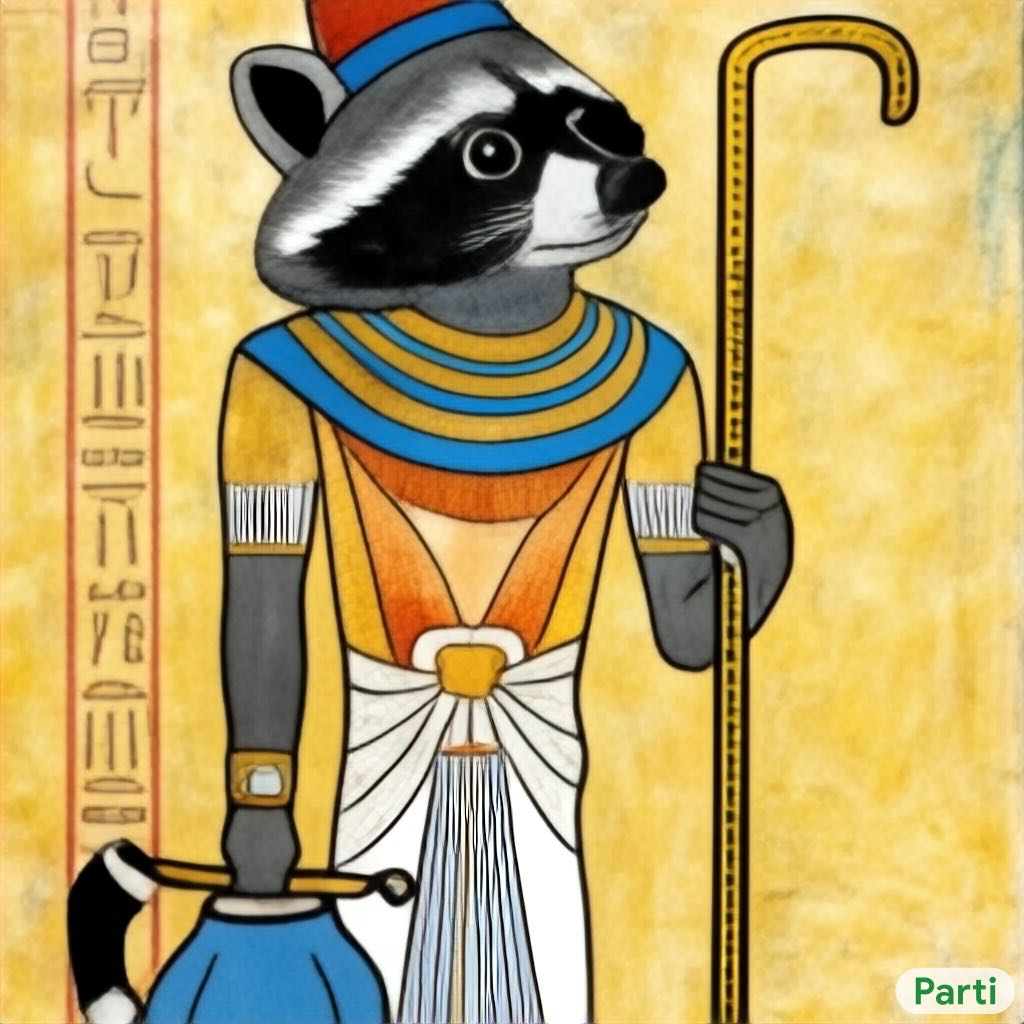
\includegraphics[width=\threebythreecolwidth\textwidth]{figures/cherries/egyptian.jpg}} &
\multicolumn{2}{c}{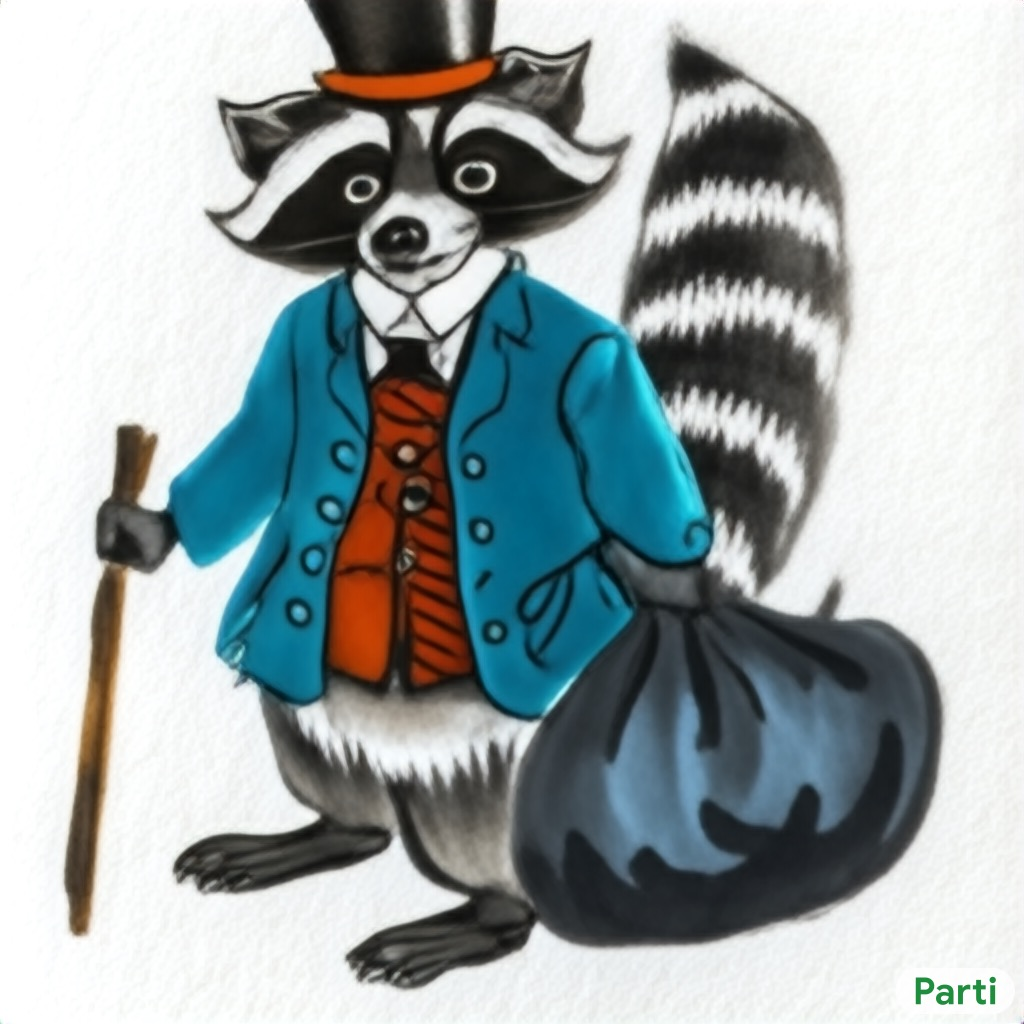
\includegraphics[width=\threebythreecolwidth\textwidth]{figures/cherries/chinese.jpg}} &
\multicolumn{2}{c}{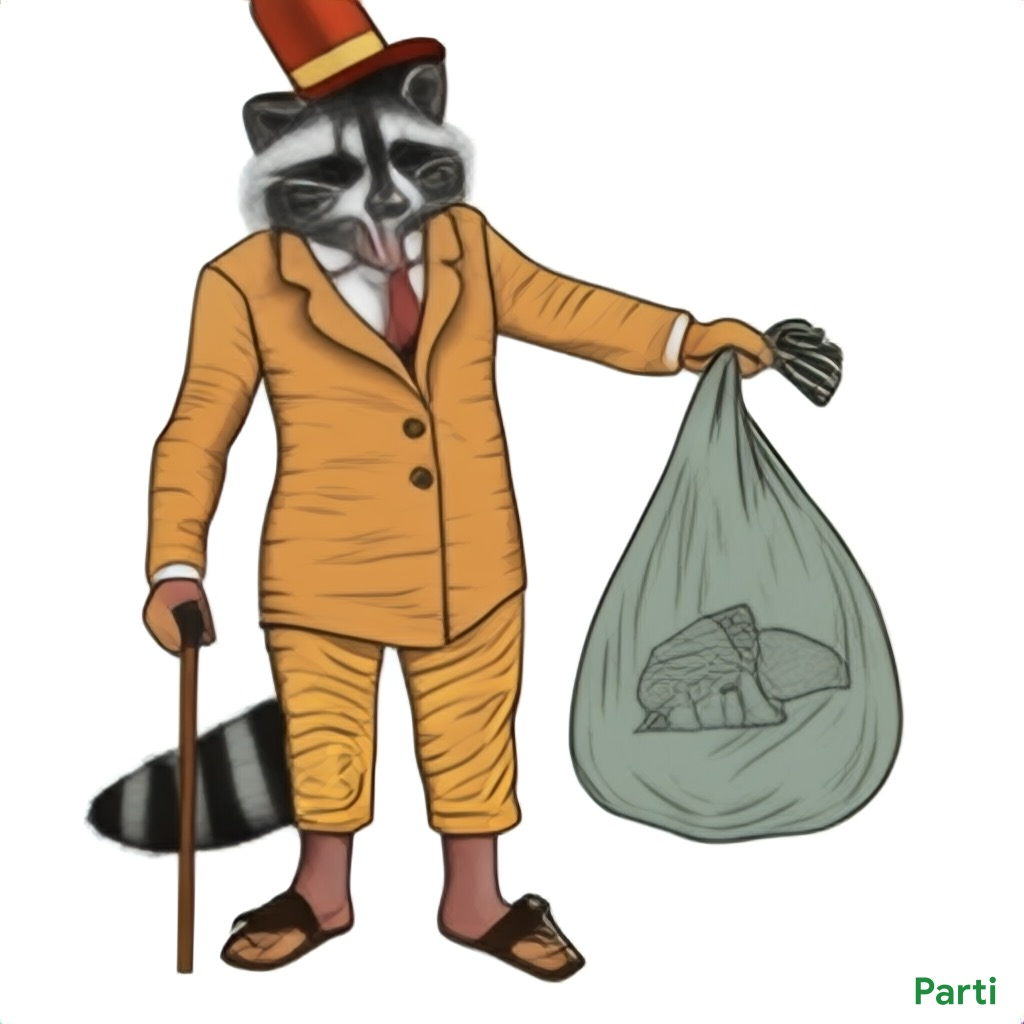
\includegraphics[width=\threebythreecolwidth\textwidth]{figures/cherries/madhubani.jpg}} &&
\multicolumn{2}{c}{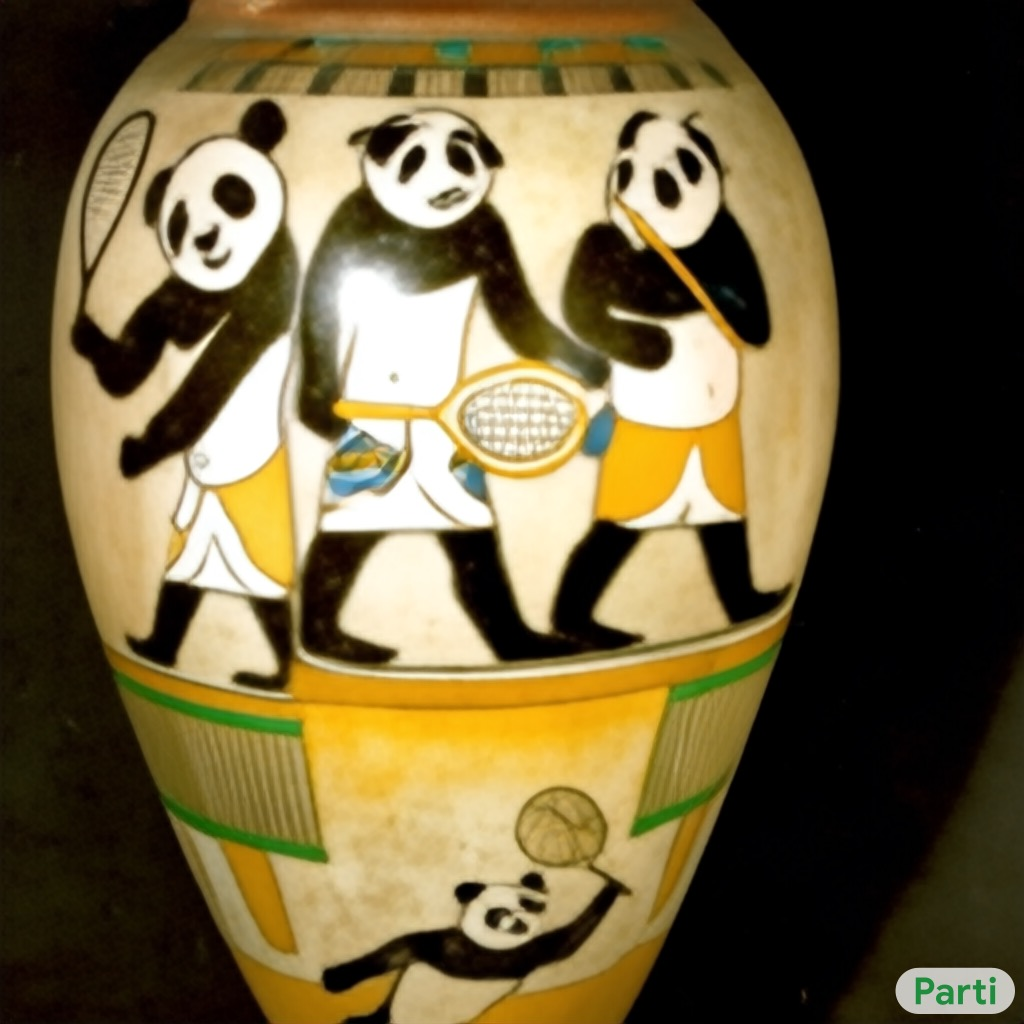
\includegraphics[width=\threebythreecolwidth\textwidth]{figures/cherries/panda_tennis.jpg}} &
\multicolumn{2}{c}{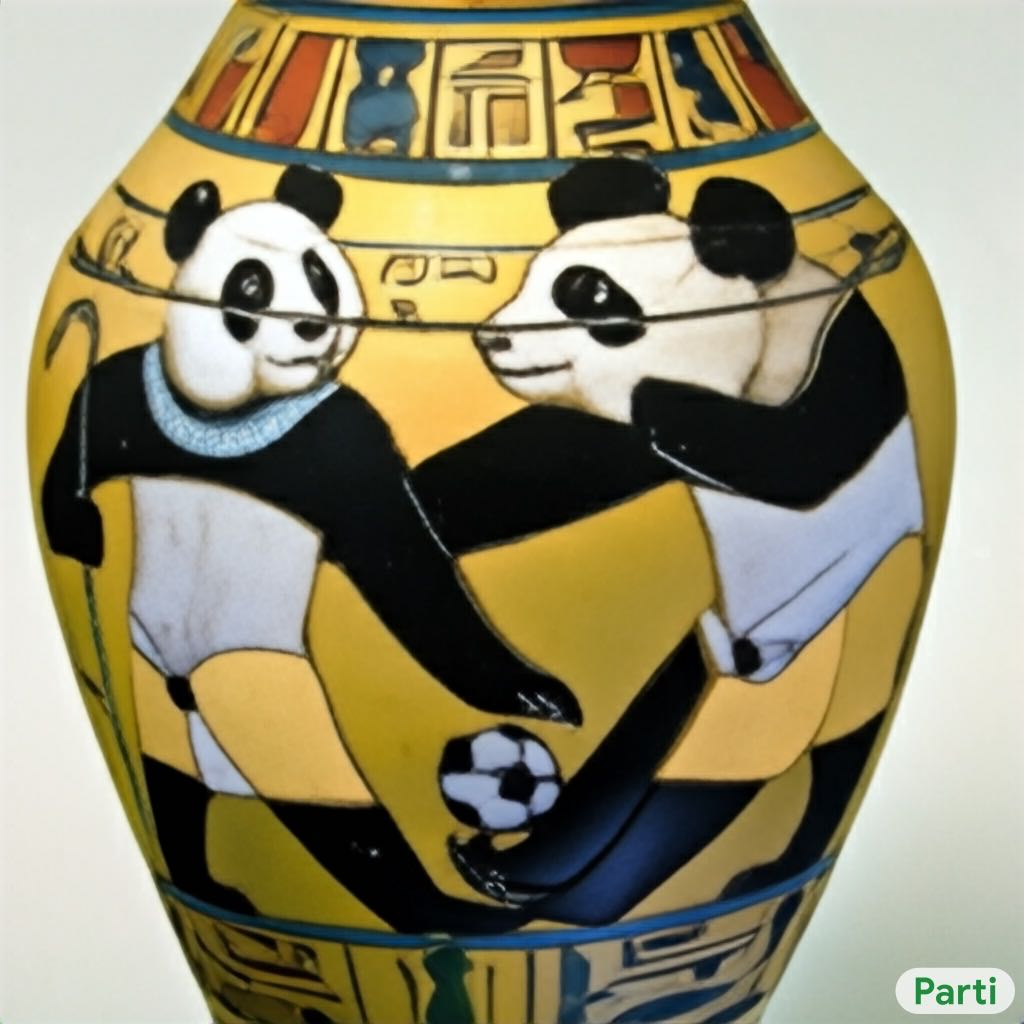
\includegraphics[width=\threebythreecolwidth\textwidth]{figures/cherries/panda_soccer.jpg}} &
\multicolumn{2}{c}{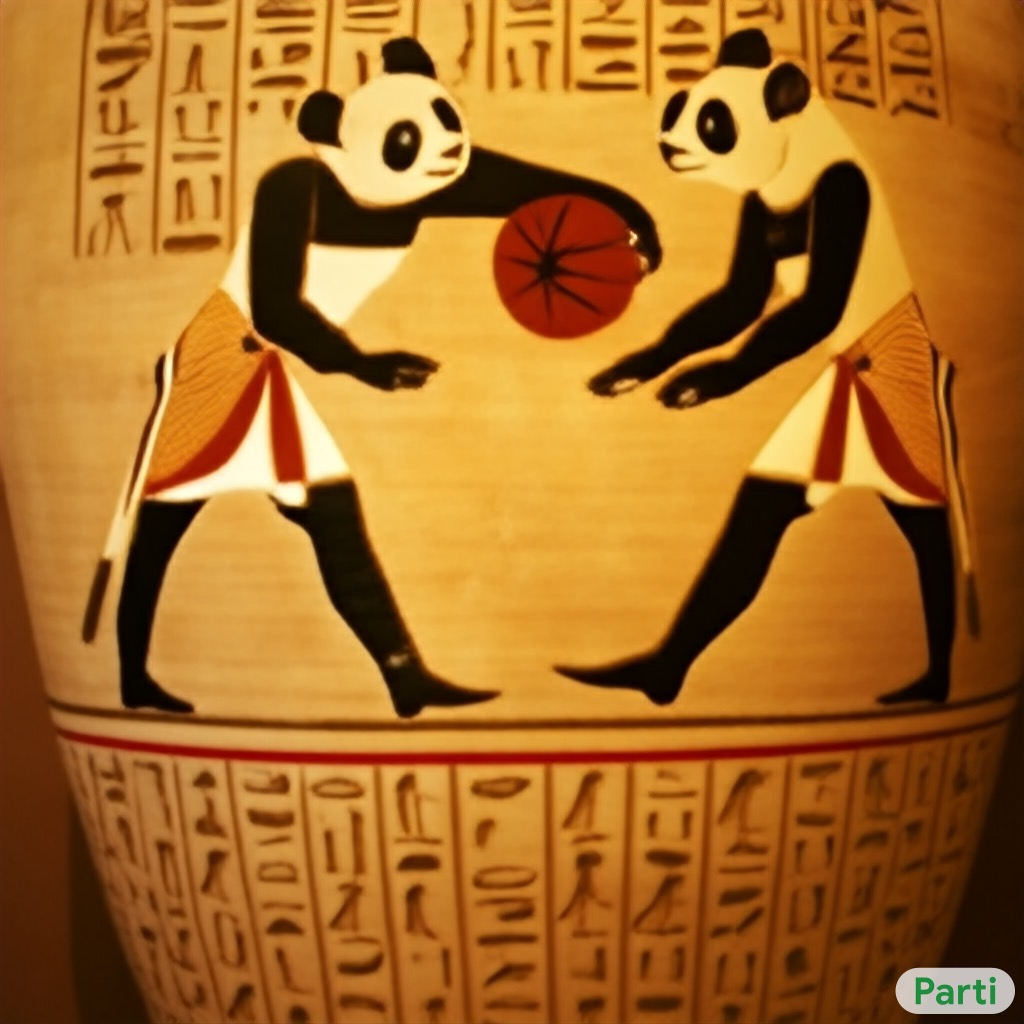
\includegraphics[width=\threebythreecolwidth\textwidth]{figures/cherries/panda_basketball.jpg}}\\

\multicolumn{6}{p{\thirdcolwidth\textwidth}}{{\tiny \textbf{G}. \textit{Three-quarters front view of a X Y Z coming around a curve in a mountain road and looking over a green valley on a cloudy day. DSLR photograph.} \textit{X} $\in$ \{\textit{blue, red, yellow}\}, \textit{Y} $\in$ \{\textit{1977, 1997, 2017}\}, \textit{Z} $\in$ \{\textit{Porsche 911, Corvette, Ford F-150}\}}} &&
\multicolumn{6}{p{\thirdcolwidth\textwidth}}{{\tiny \textbf{H}. \textit{A raccoon wearing formal clothes, wearing a tophat and holding a cane. The raccoon is holding a garbage bag. Oil painting in the style of X.} \textit{X} $\in$ \{\textit{``Rembrandt'', ``Vincent Van Gogh'', ``Hokusai'', ``pixel art'', ``pointillism'', ``abstract cubism'', ``Egyptian tomb heiroglyphics'', ``traditional Chinese painting'', ``Madhubani art''}\}}} &&
\multicolumn{6}{p{\thirdcolwidth\textwidth}}{{\tiny \textbf{I}. \textit{A photo of an Athenian vase with a painting of X playing Y in the style of Egyptian hieroglyphics.} \textit{X} $\in$ \{\textit{``pandas'', ``toucans'', ``pangolins''}\}, \textit{Y} $\in$ \{\textit{``tennis'', ``soccer'', ``basketball''}\}}} \\
\end{tabular}
\end{adjustwidth}
\caption{Selected \bdraw images. See Section \ref{sec:selected_discussion} for discussion.}
\label{figs:cherries}
\end{figure}


\section{Introduction}

People are generally able to conjure rich and detailed scenes through descriptions expressed in written or spoken language. Supporting the ability to generate images based on such descriptions can potentially unlock creative applications in many areas of life, including the arts, design, and multimedia content creation. Recent research on text-to-image generation, \eg, DALL-E~\cite{ramesh2021zero} and CogView~\cite{ding2021cogview}, has made significant progress in generating high-fidelity images and demonstrating generalization capabilities to unseen combinations of objects and concepts. Both treat the task as a form of language modeling, from textual descriptions into visual words, and use modern sequence-to-sequence architectures like Transformers~\cite{vaswani2017attention} to learn the relationship between language inputs and visual outputs. A key component of these approaches is the conversion of each image into a sequence of discrete units through the use of an image tokenizer such as dVAE~\cite{rolfe2016discrete} or VQ-VAE~\cite{van2017neural}. Visual tokenization essentially unifies the view of text and images so that both can be treated simply as sequences of discrete tokens---and thus amenable to sequence-to-sequence models. To that end, DALL-E and CogView employed decoder-only language models, similar to GPT~\cite{radford2018improving}, to learn from a large collection of potentially noisy text-image pairs~\cite{changpinyo2021cc12m, align-paper}. Make-A-Scene~\cite{gafni2022make} further expands on this two-stage modeling approach to support both text and scene-guided image generation.

A different line of research with considerable momentum involves diffusion-based text-to-image models, such as GLIDE~\cite{nichol2021glide} and concurrent works DALL-E 2~\cite{ramesh2022hierarchical} (\aka, unCLIP) and Imagen~\cite{imagen}. These models eschew the use of discrete image tokens in favor of diffusion models~\cite{ho2020denoising, dhariwal2021diffusion} to directly generate images. These models improve zero-shot Fr\'echet Inception Distance (FID) scores on MS-COCO~\cite{lin2014microsoft} and produce images of markedly higher-quality and greater aesthetic appeal compared to previous work. Even so, autoregressive models for text-to-image generation remain appealing given extensive prior work on scaling large language models~\cite{gpt3, lamda, du2021glam, palm} and advances in discretizing other modalities--such as images and audio--so that inputs in those modalities can be treated as language-like tokens. This work presents the Pathways Autoregressive Text-to-Image (\textit{\bdraw}) model, which generates high-quality images from text descriptions, including photo-realistic ones, paintings, drawings, and more (see Fig.\ \ref{figs:teaser} \& \ref{figs:cherries}). We show that with a ViT-VQGAN~\cite{yu2021vector} image tokenizer, scaling autoregressive models is an effective way to improve text-to-image generation, enabling such models to accurately integrate and visually convey world knowledge.

\bdraw is a sequence-to-sequence model based on the Transformer~\cite{vaswani2017attention}, an architecture critical to performance on many tasks, including machine translation~\cite{vaswani2017attention}, speech recognition~\cite{zhang2020transformer, gulati2020conformer}, conversational modeling~\cite{meena}, image captioning~\cite{yu2022coca}, and many others. \bdraw takes text tokens as inputs to an encoder and autoregressively predicts discrete image tokens with a decoder (see Figure~\ref{figs:overview}).
The image tokens are produced by the Transformer-based ViT-VQGAN image tokenizer~\cite{yu2021vector}, which produces higher-fidelity reconstructed outputs and has better codebook utilization compared with dVAE \cite{rolfe2016discrete}, VQ-VAE \cite{van2017neural}, and VQGAN~\cite{Esser21vqgan}. \bdraw is conceptually simple: all of its components -- encoder, decoder and image tokenizer -- are based on standard Transformers~\cite{vaswani2017attention}. This simplicity makes it straightforward to scale our models using standard techniques and existing infrastructure~\cite{megatron, du2021glam, palm, xu2021gspmd}. To explore the limits of this two-stage text-to-image framework, we scale the parameter size of \bdraw models up to 20B, and observe consistent quality improvements in terms of both text-image alignment and image quality. The 20B \bdraw model achieves new state-of-the-art zero-shot FID score of \fid{} and finetuned FID score of \fidft{} on MS-COCO.

While most recent work has focused exclusively on the MS-COCO benchmark, we also show that strong zero-shot and finetuned results can be achieved on the Localized Narratives dataset~\cite{PontTuset_eccv2020}, which has descriptions that are four times longer than MS-COCO's on average. These results demonstrate the strong generalization capability of \bdraw to longer descriptions, allowing us to pile on considerable complexity in our explorations with the model (see examples in Figure~\ref{figs:cherries} and the Appendix, and the discussion of \textit{growing a cherry tree} in Section~\ref{secs:growing_cherry_tree}). Nevertheless, existing captioning / descriptioning datasets are limited to photographs and descriptions of their contents, but much of the appeal of text-to-image models is that they can produce novel outputs for fantastical prompts. Given this, we introduce {\it \bcp{}} (\bcpa{}), a rich set of over \bcpsize{} (English) prompts curated to measure model capabilities across a variety of categories and controlled dimensions of difficulty.\footnote{Imagen \cite{imagen} introduces 200 prompts in DrawBench for similar purposes. See Section \ref{secs:bcp} for discussion.} Each prompt in \bcpa{} is associated with both a broad category (out of \bcpcat{} categories, ranging from abstract to animals, vehicles, and world knowledge) and a challenge dimension (out of \bcptrick{} aspects, ranging from basic, to quantity, words \& symbols, linguistics, and complex). Our detailed analyses and human evaluations on MS-COCO, Localized Narratives and \bcpa{}, along with extensive discussion of \bdraw's limitations (Section \ref{secs:limitations}) give a comprehensive picture of the strengths and weaknesses of \bdraw models---and establish autoregressive models as strong contenders for high-quality, broadly capable, open-domain text-to-image generation models.

Our main contributions include: (1) We demonstrate that autoregressive models can achieve {\it state-of-the-art} performance: 7.23 zero-shot and 3.22 finetuned FID on MS-COCO, and 15.97 zero-shot and 8.39 finetuned FID on Localized Narratives; (2) {\it Scale matters}: our largest \bdraw{} model (20B) is most capable at high-fidelity photo-realistic image generation and supports content-rich synthesis, particularly those involving complex compositions and world knowledge; and (3) We also introduce a holistic benchmark, the {\it \bcp{}} (\bcpa{}), propose a novel concept of {\it \cherry{}}, establish a new precedent regarding identifying limitations of text-to-image generation models, and provide a detailed breakdown, with exemplars, for error types we observed.